% Chapter Template

\chapter{Non-thermal emission from compact object merger} \label{ch:afterglow} 

In this chapter we consider non-thermal \ac{EM} counterparts of \ac{BNS} 
mergers, the \ac{SGRB} and \ac{kN} afterglows.





\section{$\gamma$-ray bursts and kilonova afterglows}

\acp{GRB} are irregular pulses of gamma-ray radiation with broken power-law 
(non-thermal) spectrum, peaking at KeV-MeV \citep{Band:1993,Kouveliotou:1993,Meegan:1992xg}.
%
With respect to the duration, \ac{GRB} are split into two categories: \ac{SGRB}, 
that last ${\leq}2$~s and long \ac{GRB} that last ${\gtrsim}2$~s. The latter are the 
result of the collapse of massive ${\geq}15M_{\odot}$ stars, while the former, at 
least in part, is attributed to mergers of compact objects. Only very recently it 
was directly confirmed with the detection of \ac{SGRB} \GRB{} that accompanied 
the \ac{GW} event \GW{} \citep{TheLIGOScientific:2017qsa}. However, the exact physical 
origin of different duration \ac{GRB} is not fully understood.
%
Indications that long \ac{GRB} are associated with core-collapse supernovae, \acp{SN}, 
are two fold. These \acp{GRB} are typically observed in star-forming regions of their 
host galaxies \citep[\eg][]{Bloom:2000pq,Bloom:2002hc,Fruchter:2006py,Christensen:2004yx,CastroCeron:2006jh} 
and several \acp{GRB} are spectroscopically associated with Type Ic \acp{SN}, albeit 
these \acp{GRB} were significantly less bright and might not be typical \acp{GRB} 
\citep[\eg][]{Liang:2006ci,Bromberg:2011fm}. Additionally, the late time behaviour 
of some \acp{GRB} includes a \acp{SN}-like "bump" in the optical and spectral changes 
that might imply that underlying \acp{SN} flux becomes dominant over \acp{GRB} 
\citep[\eg][]{Bloom:1999,Woosley:2006fn}.
%
The \acp{GRB} are distant events, most of which were localized to outside the local 
group \citep[\eg][]{Mao:1992,Piran:1992,Fenimore:1993}. Particularly useful for distance 
estimation were the observations of \ac{GRB} afterglow, fading X-ray \& optical emission, 
that allow to estimate the redshift \citep[\eg][]{Costa:1997cg,Frontera:1997ae}.
%
Analysis of the multi-wavelength afterglow data for \acp{GRB} \citep[\eg][]{Panaitescu:2001bx} 
suggested the mechanism behind the afterglow emission is the synchrotron radiation from the 
external forward-shock, which forms when \ac{GRB}-ejecta sweeps-up the \ac{CBM} or \ac{ISM}
medium\footnote{
    The specific indications are the power law decay of the light curves, 
    $F_{\nu}\propto^{-1}$ and power-law spectrum $F_{\nu}\propto\nu^{-0.9\pm 0.5}$.
} 
\citep{Rees:1992ek,Paczynski:1993gz,Meszaros:1993ju,Meszaros:1996sv}.
%
The temporal behavior of many (but not all) \acp{GRB} shows a change, a steepening 
of the light-curve (to $F_{\nu}\propto t^{-2.2}$) at $\sim 1$~day after the burst. 
This is usually attributed to the 
%\gray{deceleration of the colimated GRB-outflow, jet, and decrease on the realtivisitc beaming. This in turn makes the edge of the jet visible to an observer.} 
finite angular extend of the \ac{GRB}-ejecta, jet \citep[\eg][]{Rhoads:1999wm,Sari:1999mr}. 
When jet decelerates and relativistic beaming decreases (and the jet edge becomes visible), 
the optical and X-ray lightcurves decay achromatically faster. This achromatic transition 
from slow to faster decay is called "jet-break".
%
%%% PROBLEMO -- jet-break is not a universal feature.
%Notably, this jet-break is not observed in all \acp{GRB} for the reason that is not fully 
%understood \citep[\eg][]{Fan:2006pj,Panaitescu:2006,Liang:2007ti,Sato:2006jg,Liang:2007rn,Curran:2007cp,Racusin:2008bx}
%%
%%% PROBLEMO -- GRB density seems uniform, but SSE models predict wind-like profile
%Models of the broadband emission of \acp{GRB} with jet-break showed that the 
%\ac{CBM}, is uniform with number density \red{$\sim 10^{-3}$} \citep{Panaitescu:2001bx}. 
%If \acp{GRB} produced in collapse of massive stars \citep{Woosley:1993,Paczynski:1997yg}, 
%this contradicts the expected density profile from stellar winds, \eg, $\rho\propto r^{-2}$ 
%\citep[\eg][]{Dai:1998iz,Chevalier:1999jy,Chevalier:1999mi,Ramirez-Ruiz:2001} 
%\red{this might be very outdated.}
%
%% sGRB
The origin of \acp{SGRB} was first connected with the elliptical galaxes, and with 
older stellar population 
\citep[\eg][]{Gehrels:2005qk,Fox:2005kv,Barthelmy:2005bx,Berger:2005dr,Panaitescu:2005er,Bloom:2005qx,Guetta:2005bb,Nakar:2007yr} 
and thus with \ac{BNS} mergers. A more direct evidence came with the \GRB{}
\citep{Savchenko:2017ffs,Alexander:2017aly,Troja:2017nqp,Monitor:2017mdv,Nynka:2018vup,Hajela:2019mjy}, 
detected by the space observatories Fermi \citep{TheFermi-LAT:2015kwa} and INTEGRAL \citep{Winkler:2011}.
%
Generally \acp{SGRB} show a complex time behavior of early afterglow X-ray emission, 
in particular a presence of a plateau ($F_{x}\propto t^{-1/2}$), after the initial sharp 
decrease ($F_{x}\propto t^{-3}$) which a standard forward shock model does not predict. 
This implies that early X-ray afterglow is shaped by a variety of physical processes 
\citep{Zhang:2005fa}.
%
The \GRB{} was dimmer then any other events of its class. 
Different interpretations for its dimness and slow rising flux were proposed: off-axis jet, 
cocoon or structured jet. Now it is commonly accepted that \GRB{} was a structured jet 
observed off-axis 
\citep[\eg][]{Fong:2017ekk,Troja:2017nqp,Margutti:2018xqd,Lamb:2017ych,Lamb:2018ohw,Ryan:2019fhz,Alexander:2018dcl,Mooley:2018dlz,Ghirlanda:2018uyx}.
The \GRB{} late emission, the afterglow, provided information on 
the energetics of the event and on the properties of the circumburst medium 
\citep[\eg][]{Hajela:2019mjy}. 

%%%% EARLY emission problem
%Two main questions stem from these observations: is the mechanism behind the prompt 
%$\gamma$-ray emission and early afterglow emission is the same (or do they originate from 
%the same outflow), and is the early X-ray radiation produced by the external shock (just a 
%blast wave takes long time to become self-similar) or does it originate from an internal 
%shock? An indication that the long-lived central engine activity might affect the 
%afterglow came from the observed sharp increase in X-ray flux (flares) on a 
%scale of minutes to hours after the end of the \ac{GRB}
%\citep{Burrows:2005ww,Chincarini:2007fp,Chincarini:2010,Margutti:2011}, 
%which could not be attributed to the inhomogeneities in the \ac{CBM}.
%%% PROBLEMO!
%Thus, the early X-ray behaviour of \acp{GRB} $t < 10^{4}$~s post-burst is not well 
%understood and seems to be in tension with standard afterglow forward shock emission model.

%\textcolor{red}{
%    One of the foremost unanswered questions about GRBs is the physical mechanism
%    by which prompt $\gamma$-rays the radiation that triggers detectors on board
%    GRB satellites are produced. Is the mechanism the popular internal shock
%    model 6 \cite{(Rees and Meszaros, 1994)}, the external shock model, or something
%    entirely different? Are $\gamma$-ray photons generated via the synchrotron process
%    or inverse-Compton process, or by a different mechanism? Answers to these
%    questions will help us address some of the most important unsolved problems
%    in GRBs  how is the explosion powered in these bursts? Does the relativistic
%    jet produced in these explosions consist of ordinary baryonic matter, electron positron
%    pairs, or is the energy primarily in magnetic fields?
%}

%Once again, while it is suggested that the high energy emission, after the propmt phase is produced 
%by the synchrotron process in the external forward shock, \citep{Kumar:2009,Ghisellini:2010}, 
%the mechanism behind the high and low energy $\gamma$-ray emission in the prompt phase remains unknown. 
%Possible mechanisms include: inverse Compton and synchrotron emission in internal and external shocks
%\citep[\eg][]{Rees:1992ek,Dermer:1998py,Lyutikov:2003ih,Zhang:2011} and 
%photospheric radiation with contribution from multiple \ac{IC} scatterings
%\citep[\eg][]{Thompson:1994zh,Ghisellini:1998jy,Meszaros:1999gb,Peer:2005qoc,Peer:2008udu,Giannios:2006jb,Ioka:2007qk,Asano:2009gi,Lazzati:2010,Beloborodov:2010,Toma:2011}.

%% from the Afterglow paper



%\subsection{kilonova afterglow}

In addition to the \ac{GRB} beamed emission, the non-thermal, more isotropic 
emission is expected from electrons accelerated in shocks formed between the 
(mildly) relativistic ejecta and the \ac{ISM} \citep{Nakar:2011cw}. This emission 
is expected to peak in radio band and continue on a time scale of tens of years 
after merger. Notably, all ejecta components will contribute to the emission, 
but depending on the ejecta velocities and kinetic energy, 
the brightness in different frequencies and timescales differs. 
%
Various ejecta components interact with each other and with \ac{ISM}. The latter, 
generates a long-lived blast wave. The shock, propagating upstream, amplifies 
(random) magnetic fields and accelerates electrons, that subsequently emit 
synchrotron radiation. This process in phenomenological similar to the for the 
\ac{GRB} afterglow and \ac{SN} early remnants. 
%
Numerical simulations of \ac{BNS} mergers showed the presence of mildly relativistic 
ejecta (See Sec.~\ref{sec:bns_sims:method:ejecta}). 
Several studies on the possible non-thermal electromagnetic emission of this ejecta 
have been carried out 
\citep[\eg][]{Piran:2012wd,Hotokezaka:2015eja,Hotokezaka:2018gmo,Radice:2018pdn}. 
Notably, the observed non-thermal emission from \GW{}, was first interpreted 
as the non-thermal emission from the ejecta \citep{Mooley:2017enz}.
This interpretation was however disproved by the emergence of jet break
%
%Specifically, a strong radio emission is expected from \ac{BNS} ejecta \citep{Piran:2012wd,Hotokezaka:2015eja}. 
The \ac{BNS} merger radio remnant is expected to peak on a time-scale 
of years after the merger and be visible over a similar timescale. Notably, this is 
assuming that the ejecta is expanding into the unshocked \ac{ISM}, as it was shown 
that if the \ac{ISM} is pre-shocked by the jetted outflow, and the \ac{ISM} density is 
reduced, the kilonova afterglow would be delayed. 
%
In \citet{Piran:2012wd}, the synthetic \ac{kN} afterglow \acp{LC} are calculated 
for a set of \ac{NR} \ac{BNS} merger simulation with properties typical to the 
Galactic binary population and \ac{ISM} density usually found in the Galactic disk, 
$\nism\sim1\ccm$. Authors showed that the from a binary of two $1.4\Msun$ \acp{NS}, 
the kilonova afterglow would peak $\sim10$~years after the merger if $\nism = 0.1\ccm$ 
and $\sim3$~years if $\nism = 1\ccm$ in radio bands, $\nu=1.4$~GGz and $\nu=150$~MGz. 
Notably, both values of the \ac{ISM} density are larger than what is inferred for \GW{}. 
Indeed, jet fitting models and dependent analysis of the diffuse emission suggest 
$\nism\in(10^{-4},10^{-2})$\gcm \citep{Hajela:2019mjy}.
%In \citet{Piran:2012wd} authors focus on the observational prospects of this afterglow 
%and compare it to other \ac{EM} emission expected for \ac{BNS}. 


%\red{motivation why it is important to model nucleosynthesis}
%
%
%\red{Subsection of GRBs}
%\cite{Lee:2007js,Nakar:2007yr,Gehrels:2009,Fernandez:2015use}





\section{Afterglow theory}

\red{Based in the \cite{Kumar:2014upa} work}.
In this section we outline of the most relevant physical processes in \ac{GRB}
and \ac{kN} afterglows. It is not meant as a comprehensive theoretical review. 
For this we refer the interested reader to the momnograph by \citet{RybickiLightman:1985}, 
as well as books of high energy astrophysics by \citet{Longair:2011,Dermer:2009}.


\subsection{Special relativistic effects}

Consider a moving source of radiation and an observer with a line of sight to the source.
Let $\upsilon$, $\Gamma$ and $\theta$ be the source velocity, 
\ac{LF} and angle with the line of sight.
%
Consider three frames of reference, the comoving frame (usually denoted with a prime $'$),
the lab frame, where the source is seen as moving with $\upsilon$ and observer frame.
Then, if two photons are emitted in the comoving frame with time difference of $\delta t'$,
which is in the lab frame $\delta t = \Gamma \delta t'$, the observer sees the two 
photons arrive with 
%
%\begin{eqnarray}
%\delta t_{obs} &= \delta t + \frac{(d - \upsilon\cos(\theta) \delta t)}{c} - \frac{d}{c} \\
%&= \delta t (1 - \upsilon \cos(\theta) / c) \\
%&= \delta t' \Gamma (1 - \upsilon \cos(\theta) / c)\\
%&= \delta t' \mathcal{D}^{-1}
%\end{eqnarray}
%
$\delta t_{obs} = \delta t' \mathcal{D}^{-1}$
%
where $d$ is the distance to the source, and 
%
\begin{equation}
\mathcal{D} = \frac{1}{\Gamma(1 - (\upsilon/c) \cos(\theta))} = \frac{1}{\Gamma(1 - \beta\cos(\theta))}
\label{eq:afterglow:dop_fac}
\end{equation}
%
is the \ac{DF}. 


Next, we consider the transformation of the photon frequencies. 
%
The Lorentz transformation of the photon $4$-momentum in comoving frame, \eg,, 
$\nu'(1, \cos(\theta'), \sin(\theta'),0)$ to the lab frame $4$-momentum 
$\nu(1, \cos(\theta), \sin(\theta), 0)$
%
%\begin{equation}
%\nu = \nu' \Gamma(1+\upsilon \cos(\theta')/c) \text{ \& } \nu\cos(\theta) = \nu' \Gamma (\cos(\theta') + \upsilon/c)
%\end{equation}
%%
%or 
%
\begin{equation}
\nu = \frac{\nu'}{\Gamma (1 - \upsilon\cos(\theta)/c)} = \nu' / \mathcal{D}
\label{eq:afterglow:dop_fac_freq}
\end{equation}
%
%which is a standard Doppler shift formula.



%\subsubsection{Relativistic beaming of photons}

%%%% ---------------------------------------
%%%% --- On the Angular size of the source
%%%% ---------------------------------------
%
%We have shown that $\nu = \nu' \mathcal{D}$, but also 
%$\sin(\theta) = \sin(\theta')/\mathcal{D}$. Then the transverse component of the 
%momentum is invariant under the Lorentz transformation, \eg, 
%$\nu_{\perp}' = \nu'\sin(\theta') = \nu\sin(\theta) \nu_{\perp}$. 
%%
%For a beam of photons it implies that the angular size of the beam is smaller 
%in the lab frame than in the comoving frame by $\propto \Gamma$.
%%
%The solid angle of a conical beam of photons, $d\Gamma$ then 
%%
%\begin{equation}
%d\Gamma = \sin(\theta)d\theta d\phi = \sin(\theta') d\theta' d\phi' / \mathcal{D}^2 = d\Omega'/\mathcal{D}^2
%\end{equation}
%%
%is smaller in the lab frame than in the comoving frame.
%%
%Next, consider a frequency integrated total energy radiated per 
%unit time over the $4\pi$ steradians, denoted as $P$. 
%%
%The power in the lab frame $P = P'\Gamma\delta t'/(\Gamma\delta t') = P'$. 
%Hence, power radiated by particles is \magenta{Lorentz invariant}.

%%%% -------------------------------------------------------------
%%%% Transformation of specific luminosity and specific intensity
%%%% -------------------------------------------------------------
%
%Consider a spherically symmetric source, expanding with \ac{LF} $\Gamma$.
%%
%The \magenta{specific luminosity} is defined as the total energy that passes 
%through the surface enclosing the source per unit time, per unit frequency, 
%$L_{\nu} = dE / d\nu dt_{obs}$. 
%As $d\nu dt_{obs} = d\nu' dt'$ and $E=\Gamma E'$, the Lorentz transformation 
%of luminosity is
%%
%\begin{equation}
%L_{\nu} = \frac{dE}{d\nu dt_{obs}} = \Gamma \frac{dE'}{d\nu' dt'} = \Gamma L_{\nu}'
%\end{equation}
%%
%assuming that the $3$-momentum is zero (as the source is spherically symmetric).
%%
%The \magenta{specific intensity} is defined as a flux per unit frequency 
%and per unit solid angle, mediated by photons, traversing surface $dA$, 
%perpendicular to the conical beam, confining the photons, 
%%
%\begin{equation}
%I_{\nu} = \frac{dE}{d\nu dt_{obs} dA d\Omega}
%\end{equation}
%%
%that has a Lorentz transformation $I_{\nu} = \mathcal{D}^3 I_{\nu'}'$ 
%as $d\nu dt_{obs} dA$ is the Lorentz invariant.

%%%% ------------------------------------------------------------
%%%% Observed \ac{LC} from a source that is suddenly turned off
%%%% ------------------------------------------------------------
When considering the extended source that suddenly turns off, the observed emission, 
due to the final size of its origin, does not shuts down, but steeply declines and can 
be computing integrating over the \ac{EATS}.
%
Consider a thin shell with a point, characterized by $(r, \theta, \phi)$ where $\theta$ 
is the angle measured with respect to the line of sight to the observer. Then, photons, 
emitted at $(r=\upsilon t, \theta,\phi)$ arrive at the observer with a time delay with 
respect to a photon emitted at $r=0$ of
%
\begin{equation}
t_{obs} = t - \frac{r \cos(\theta)}{c} = t(1-\frac{\upsilon\cos(\theta)}{c}) = \frac{t}{\Gamma\mathcal{D}}
\label{eq:afterglow:tobs}
\end{equation}


Now, consider the observed emission from the source at frequency $\nu$. 
The starting time is $t_{0;obs}\approx(R_0 2 c \Gamma^2)$, \red{check!} 
at which photons, emitted from $(R_0, 0, 0)$ arrive, At later times, 
$t_{obs}>t_{0;obs}$, the observer still sees photons emitted when $r < R_0$. 
%
Assume that the intrinsic emission spectrum is $I_{\nu'}' = I'\nu^{'-\beta}$.
Then, at $t_{obs} > t_{0;obs}$ the radiation from $\theta > \theta_t$ 
(where $\theta_t$ corresponds to $t_{obs} = R_0 (1/\upsilon - \cos(\theta_t)/c)$) 
reaches the observer.
%
The observed flux \eg, $f_{\nu} \propto \int I_{\nu} d\Omega$, has the following 
Lorentz transformation 
$f_{\nu}\propto\int_{\theta_t} d\theta \sin(\theta_t) \mathcal{D}^{-(3+\beta)}$.
%
%%%% ---------------------------
%%%% A More Regorous Derivation
%%%% ---------------------------
%Now, consider a more rigorous derivation of the transformation of the specific 
%flux in observer frame from relativistic source with comoving specific intensity 
%$I_{\nu'}'$ and spectrum $\propto \nu^{' -\beta}$
%%
%\begin{equation}
%f_{\nu}(t_{obs}) = \int d\Omega_{obs} I_{\nu} \cos(\theta_{obs}) = 2\pi \int d\theta_{obs} \frac{ I_{\nu'_0}' \nu_{0}^{'\beta}\sin(2\theta_{obs})[(1+z)\Gamma]^{-(3+\beta)} }{ 2\nu^{\beta} [ 1-\upsilon\cos(\theta + \theta_{obs}) / c ]^{3+\beta} }
%\end{equation}
%%
%where $\nu_0 '$ is a frequency that lies on the power law segment of the spectrum for 
%$I_{\nu'}'$. The Lorentz transformation of the specific intensity was made above. 
%The factor $(1+z)^{3+\beta}$ accounts for the Redshift on the frequency. 
%%
%Assuming that $\sin(\theta)/d_{A} = \sin(\theta_{obs})/r$, the above integral writes 
%%
%\begin{equation}
%f_{\nu} \approx \frac{ 2\pi I' \nu' _0 \nu_{0}^{'\beta}\nu^{-\beta} }{[(1+z)\Gamma]^{3+\beta}} \Big( \frac{R_0}{d_A} \Big)^2 \int_{\theta_t}^{\pi / 2} d\theta \frac{\sin(\theta)\cos(\theta)}{(1-\upsilon\cos(\theta)/c)^{3+\beta}},
%\end{equation}
%where $\theta+\theta_{obs}$ in the denominator was replaced with $\theta$ as $\theta_{obs}\ll\theta$.
%The integral is simple to compute. Ir yields
%
%\begin{equation}
%f_{\nu}(t_{obs}) \propto (1 - \upsilon\cos(\theta_t)/c)^{-(2 + \beta)}\nu^{-\beta} \propto t_{obs}^{-(2+\beta)} \nu^{-\beta},
%\end{equation}
%%
%This equation shows, that the observed radiation does not immediately turns off 
%when the source switches off. The flux falls off rapidly with time and vanishes 
%when $\theta_t$ exceeds the angular size of the source $(\theta_j)$.
%
%
%The \ac{EATS} integration can be performed as follows.
%The expanding thin shell is composed of infinitesimal elements,
%each of which is evolved within its own $(d\phi, d\theta)$
%cell, center of which has coordinates $(\phi_c, \theta_c)$.
%%
%Then for each cell, the observational angle, $\mu$, is computed as 
%%
%\begin{equation}
%    \cos(\mu) = \sin(\alpha) \sin(\theta_c) \sin(\phi_c) 
%     + \cos(\alpha) \cos(\theta_c).
%\end{equation}
%%
%Then the radiation at time $t$ is observed if $t_{obs}$
%%
%\begin{equation}
%    t_{obs} = t_{lab} +\frac{r}{c}(1 - \cos{\mu})
%\end{equation}
%%
%where 
%%
%\begin{equation}
%    t_{lab} = \int \frac{1}{\beta c} dr
%\end{equation}
%%
%is the time measured in the laboratory frame of reference.
%%
%Then we interpolate the part of the dynamical evolution
%of the infinitesimal jet that corresponds to this $t_{obs}$,
%and emitted the radiation during this time.
%The flux, $F_i$, for a given Doppler-shifted frequency, 
%$\nu_{obs}'$, is then obtained for each infinitesimal segment.
%Integrating over the $F_i$ we obtain the total flux emitted by the 
%blast wave and observed at time $t_{obs}$





\subsection{Synchrotron radiation}

%Consider an electron moving in the magnetic field, perpendicular to the 
%field lines. Let $\gamma_e$, $\upsilon_e$ be the electron's \ac{LF} and 
%velocity and $B$ the magnetic field strength.
%%
%The electric field in the electron rest-frame is $E=\gamma_e \upsilon_e B /c$. 
%The electron acceleration in this field yields radiation, total power of which, 
%according to the Larmor's formula, 
%%
%\begin{equation}
%P_{syn} = \frac{2q^4E^2}{3c^3m_e}=\frac{2q^4B^2\gamma_e^2\upsilon_e^2}{3c^5m_e^2} = \frac{\sigma_TB^2\gamma_e^2\upsilon_e^2}{4\pi c}
%\end{equation}
%%
%where $\sigma_T = 8\pi q^4 / (3m_e^2c^4)$ is the Thompson cross section. 
%%
%The $P_{syn}$ is the Lorentz invariant 
%(as electric dipole radiation is Lorentz invariant).
%%
%Note, that for an isotropic pitch angle distribution, 
%the average power $\langle P_{syn} \rangle = (2/3)P_{syn}$.
%%
%The angular speed of the electron (\eg its Larmor frequency), is
%%
%\begin{equation}
%\omega_L = \frac{q B}{\gamma_e m_e c}
%\end{equation}
%%
%Within the magnetic field, an electron is moving on a spiral trajectory. 
%The relativistic beaming of emitted radiation leads to a distant observer 
%being able to see this radiation, only when the electron velocity vector is 
%within $\angle \sim \gamma_e^{-1}$ from the line of sight. Correspondingly, 
%only a fraction of orbital time, $t\sim1/(\pi\gamma_e)$, contributes to the 
%observed radiation, which appears as a repeated pulse. 
%The duration of this pulse is
%%
%\begin{equation}
%\delta t_{obs} \sim \frac{2}{\gamma_e \omega_L}\frac{1}{2\gamma_e^2}\sim \frac{m_e c}{q B \gamma_e^2}
%\end{equation}
%%
%where we used $\delta t' = \delta t / \gamma_e$. 
%%
%Then the characteristic frequency of the synchtrontron radiation is given 
%by an inverse of $\delta t$ and reads 
%%
%\begin{equation}
%\omega_{syn} \sim \frac{q B \gamma_e^2}{m_e c} \text{ and } \nu_{syn} = \frac{\omega_{syn}}{2\pi} \sim \frac{q B \gamma_e^2}{2\pi m_e c}
%\end{equation}
%%
%where $\nu_{syn}$ is the cyclic frequency.
%%
%Note that here the factor $(3/2)\sin(\alpha)$, where $\alpha$ is the pitch 
%angle between the electron's velocity and the magnetic field is \red{ommited}.
%%
%The synchrotron spectrum peaks at $\sim \nu_{syn}$. At $\nu < \nu_{syn}$ the
%$P_{syn}(\nu)\propto\nu^{1/3}$ (which is determined by the Fourier transform of 
%the synchrotron pulse profile). At $\nu > \nu_{syn}$ the power decays exponentially. 
%See \citet{RybickiLightman:1985} for the calculation of synchrotron spectrum. 
%%
%The power per unit frequency at the peak of the spectrum is given 
%%
%\begin{equation}
%P_{syn}(\nu_{syn}) \sim \frac{P_{syn}}{\nu_{syn}} \sim \frac{\sigma_T B m_e c^2}{2 q},
%\end{equation}
%
%%%% ------------------
%%%% Shortened
%%%% ------------------
%
The total emitted power of an electron, $P_{syn},$ moving with the speed $\upsilon_e$ 
(\ac{LF} $\gamma_e$) in the magnetic field, $B$, perpendicular to the field lines 
is given by Larmor's formula.
%
As within the magnetic field, an electron is moving on a spiral trajectory,
the characteristic frequency of the synchtrontron radiation, $\nu_{syn}$, is given 
by the angular speed of the electron (\eg, its Larmor frequency).
%
The power per unit frequency at the peak, $P_{syn}(\nu_{syn})$, can be computed as 
\citep{RybickiLightman:1985}
%
\begin{equation}
P_{syn} = \frac{\sigma_TB^2\gamma_e^2\upsilon_e^2}{4\pi c}, 
\hspace{5mm} 
\nu_{syn} \sim \frac{q B \gamma_e^2}{2\pi m_e c},
\hspace{5mm}
P_{syn}(\nu_{syn}) \sim \frac{\sigma_T B m_e c^2}{2 q},
\end{equation}
%
where $\sigma_T = 8\pi q^4 / (3m_e^2c^4)$ is the Thompson cross section.



%Now consider the distribution of electrons.
%Commonly adopted is the power-law distribution, $dn_e/d\gamma_e \propto \gamma_e^{-p}$, which results in emission spectrum $f_{\nu}\propto\nu^{-(p-1)/2}$,
%which is a consequence of 
%%
%\begin{equation}
%f_{\nu} = \int_{\gamma_{\nu}}^{\infty} d\gamma_e \frac{dn_e}{d\gamma_e}P_{syn}(\nu) \propto \nu^{-(p-1)/2}
%\end{equation}
%%
%as $P_{syn}(\nu) \propto (\nu/\nu_{syn})^{1/3}$ for $\nu < \nu_{syn}$\red{where is this from?}.
%%
%Here
%%
%\begin{equation}
%\gamma_{\nu} \sim \Bigg(\frac{2\pi\nu m_e c}{qB}\Bigg)^{1/2}
%\end{equation}
%%
%is the minimum \ac{LF}, above which electrons contribute to the specific flux, 
%$f_{\nu}$ \red{why?} \gray{This seems to be an equation for $\nu = f(\gamma)$ 
%    inverted, -- so is the $\nu$ a critical frequency?
%}
%
%%%% ------------------
%%%% Shortened
%%%% ------------------
%
For an ensebble of electrons with the distribution function $dn_e/d\gamma_e$, 
the emission spectrum reads 
%
\begin{equation}
f_{\nu} = \int_{\gamma_{\nu}}^{\infty} d\gamma_e \frac{dn_e}{d\gamma_e}P_{syn}(\nu) 
%\propto \nu^{-(p-1)/2}
\label{eq:afterglow:sync_power}
\end{equation}
%
where $\gamma_{\nu}$ is the minimum \ac{LF} above which electrons contribute to the 
specific flux.


%%%% ------------------------------------------------------
%%%% Effect of synchrotron cooling on electron distribution
%%%% ------------------------------------------------------

%Consider the effects of electrons cooling. 
%The characteristic frequency associated with it is $\nu_c$ and $\gamma_c$.
%Electrons with \ac{LF} $\gamma_e > \gamma_c$ can efficiently loose their energy to 
%synchrotron radiation. Then, after the time $t_0$, their $\gamma_e$ drops below 
%$\gamma_c$, 
%%
%\begin{equation}
%c^2 \frac{dm_e}{dt} \gamma_e = -\frac{\sigma_T}{6\pi} B^2 \gamma_e^2 c
%\end{equation}
%%
%\begin{equation}
%\gamma_c \sim \frac{6 \pi m_e c}{\sigma_T B^2 t_0}
%\end{equation}
%%
%The corresponding characteristic frequency is called the synchrotron cooling 
%frequency. 
%%
%\begin{equation}
%\nu_c = \frac{3}{4\pi} \gamma_c^2 \frac{q B}{m_e c}
%\end{equation}
%%
%At $\nu_c$ the spectrum of the synchrotron radiation is changing, as electrons 
%with $\gamma_e > \gamma_c$, the effects of cooling modify the electron distribution. 
%%
%%
%Consider the continuity equation for electrons in the energy space 
%%
%\begin{equation}
%\frac{\partial }{\partial t}\frac{d n_e}{d\gamma_e} + \frac{\partial}{\partial \gamma_e}\Big[ \dot{\gamma_e}\frac{dn_e}{d\gamma_e} \Big] = S(\gamma_e)
%\end{equation}
%%
%where $\dot{\gamma_e} = -\sigma_T B^2 \gamma_e^2 / (6\pi m_e c)$ is the rate at 
%which electron \ac{LF} changes due to losses, $S(\gamma_e)$ is the injection 
%rate of electrons into the system.
%%
%Assume that the minimum \ac{LF} of injected electrons is $\gamma_m$, \eg, 
%where $S(\gamma_e) = 0$ for $\gamma_e < \gamma_m$.
%Then if $\gamma_c < \gamma_e < \gamma_m$ the solution to the equation 
%$dn_{e}/d\gamma_e \propto \dot{\gamma_e}^{-1} \propto \gamma_e^{-2}$.
%%
%Then, for this electron distibution the synchrotron spectrum is 
%$f_{\nu}\propto\nu^{-1/2}$ 
%\footnote{If $B=f(t)$, then the distribution function for $\gamma_e$ 
%    evolves with time and is not a simple pwoer law with index $2$, see \citet{Uhm:2013gwa}.
%}
%%
%For $\gamma_e > \gamma_c > \gamma_m$, the solution to the equation is 
%$dn_e/d\gamma_e \propto \gamma_e^{-p-1}$ (assuming the constant $B$ field, 
%the steady state). Then the synchrotron spectrum reads $f_{\nu}\propto\nu^{-p/2}$.
%
%%%% ------------------
%%%% Shortened
%%%% ------------------
%
Depending on their \ac{LF} and the magnetic field strength, electrons can loose 
energy, cool, with different efficiency. For instance, if $\gamma_e > \gamma_c$,
where $\gamma_c$ is a certain characteristic \ac{LF}, after a finite $t_0$, the 
$\gamma_e$ will drops below $\gamma_c$, 
%
\begin{equation}
c^2 \frac{dm_e}{dt} \gamma_e = -\frac{\sigma_T}{6\pi} B^2 \gamma_e^2 c 
\, \rightarrow\, 
\gamma_c \sim \frac{6 \pi m_e c}{\sigma_T B^2 t_0}, \,
\nu_c = \frac{3}{4\pi} \gamma_c^2 \frac{q B}{m_e c}
\end{equation}
%
where $\nu_c$ is called cooling frequency. 
%
Thus, the synchrotorn spectrum differ for electrons with $\gamma_e > \gamma_c$.
%
Consider the continuity equation for electrons in the energy space 
%
\begin{equation}
\frac{\partial }{\partial t}\frac{d n_e}{d\gamma_e} + \frac{\partial}{\partial \gamma_e}\Big[ \dot{\gamma_e}\frac{dn_e}{d\gamma_e} \Big] = S(\gamma_e)
\end{equation}
%
where $\dot{\gamma_e} = -\sigma_T B^2 \gamma_e^2 / (6\pi m_e c)$ is the rate at 
which electron \ac{LF} changes due to losses, $S(\gamma_e)$ is the injection 
rate of electrons into the system.
%
Consider steady-state solution $\partial_t/\partial t = 0$.
%
Assume that the minimum \ac{LF} of injected electrons is $\gamma_m$, \eg, 
where $S(\gamma_e) = 0$ for $\gamma_e < \gamma_m$.
%Then if $\gamma_c < \gamma_e < \gamma_m$ the solution to the equation 
%$dn_{e}/d\gamma_e \propto \dot{\gamma_e}^{-1} \propto \gamma_e^{-2}$.
%%
%For $\gamma_e > \gamma_c > \gamma_m$, the solution to the equation is 
%$dn_e/d\gamma_e \propto \gamma_e^{-p-1}$ (assuming the constant $B$ field, 
%the steady state).
%
Then the electron distribution function then reads
%
\begin{equation}
    dn_e/d\gamma_e \propto 
    \begin{cases}
        \gamma_e^{-2} &\text{ if } \gamma_c < \gamma_e < \gamma_m, \\
        \gamma_e^{-p-1} &\text{ if } \gamma_e > \gamma_c > \gamma_m
    \end{cases}
    \label{eq:afterglow:elec_dist}
\end{equation}
%
with the former usually referred as \textit{slow cooling} and the latter
\textit{fast cooling} regimes.


%%%% ------------------------------------------------------
%%%% Synchrotron self-absorption frequency
%%%% ------------------------------------------------------
%If the photon absorption by the inverse-synchrotron process is important, 
%another characteristic frequency, $\nu_a$, can be determined. Consider the 
%Kirchhoff's law, \red{stating that the emergent specific flux cannot exceed the 
%    black-body flux corresponding to the appropriate electron temperature} which is
%%
%\begin{equation}
%k_BT\approx \max(\gamma_a,\min[\gamma_m,\gamma_c])m_e c^2 / 2.7
%\end{equation}
%%
%where $\gamma_m$, $\gamma_c$ and $\gamma_a$ are electron Lorentz factors 
%corresponding to $\nu_m$, $\nu_c$ and $\nu_a$.
%Then the \red{synchrotron self-absorption frequency $\nu_a$ is the 
%    frequency where the emergent synchrotron flux is equal to the black body flux
%}
%%
%\begin{equation}
%\frac{2m_ec^2\max(\gamma_a,\min[\gamma_m,\gamma_c])\nu_a^2}{2.7c^2}\approx\frac{\sigma_T B m_e c^2 N_>}{4 \pi q}
%\end{equation}
%%
%where the \ac{LHS} is the Plank function in the Rayleigh-Jeans limit and 
%$N_{>}$ is the column density of electrons with Lorentz factor larger then 
%$\max(\gamma_a\min[\gamma_m,\gamma_c])$.
%%
%Finally, the order of characteristic frequencies determines the emergent 
%synchrotron spectrum for a distribution of electrons. 
%See Fig.X for fast and slow cooling regimes \citet{Sari:1997qe}.
%
%%%% ------------------
%%%% Shortened
%%%% ------------------
%
The photon absorption by the inverse-synchrotron process can be computed by evaluating 
the black-body flux corresponding to the appropriate electron temperature 
and equating it to the emergent synchrotron flux. Alternatively, it can be accounted for 
via flux attenuation \citep{Dermer:2009}.
%

%%%% ------------------
%% Maximum energy of synchrotron photons
%%%% ------------------
%
%\subsubsection{Maximum energy of synchrotron photons}
%%
%Consider a shock front. Scattering back and forth, particles within it accelerate 
%via the \magenta{first order Fermi process}, increasing their energy $\times 2$ times, 
%at every front of the shock.
%In order to determine what is the maximum energy a particle can reach consider the 
%following. A charged particle of mass $m$ accelerates while crossing the shock front 
%on a timescale $\sim$ Larmor time, $t'_L = mc\gamma/(qB')$, where primed quantities 
%are measured in the rest frame of the fluid and $\gamma$, \ac{LF} on a particle in 
%the frame, comoving with the shock. 
%%
%The particle can accelerate to $\gamma$ only if it losses less then half of its 
%energy to synchrotron emission in $t'_L$. Then 
%%
%\begin{equation}
%\frac{4 q^4 B^{'2}\gamma^2 t'_L}{9 m^2 c^3} < \frac{m c^2\gamma}{2} \text{ or } \nu\propto \frac{q B' \gamma^2}{2\pi m c} < \frac{9 m c^3}{16\pi q^2}
%\end{equation}
%%
%Thut, for electron the maximum synchrotron photon energy is $\sim 50$~MeV and for 
%proton it is $\sim 100$~GeV in the shocked fluid comoving frame. \red{assuming 
%    Bohm diffusion limit.}
%This limit can be exceeded in case of highly inhoogeneous magnetic field 
%\citep{Kumar:2012}.
%%
%%%%% ------------------
%%% Inverse-Compton radiation
%%%%% ------------------
%%
%\subsubsection{Inverse-Compton radiation}
%
%The \ac{IC} scattering is the scattering of photons by electrons of larger energy, resulting in increase in photon energy on average.
%%% ---
%Consider electrons with $\gamma_e$ and photons with frquency $\nu$. Let $h\nu\gamma_e \ll m_e c^2$. The average frequency of scattered photons then $\nu_s\sim\nu\gamma^2_e$.
%\gray{
%    This can be seen from considering the scattering in the rest frame of the electron.
%    Let the incident photon have frequency $\nu' \sim \nu\gamma_e$. (See eq.for Doppler Shift). If $h\nu'\ll m_e c^2$, the scattering is elastic (electron recoil is negligible) and the post-scattering angle distribution is a dipol function. 
%    Then, transforming the $\nu'$ into the original frame results in $\nu_s\sim\nu\gamma_e^2$.
%}
%
%%% Single electron, Radiation Field
%Consider a radiation field with photon density $u_{\gamma}$, and an electron moving through it. 
%Then, the power in \ac{IC}-scattered photons is (assuming $h\nu\gamma_e\ll m_e c^2$)
%
%\begin{equation}
%P_{ic} \sim \sigma_T \int d\nu \frac{u_{\nu} c}{h\nu} h\nu\gamma_e^2 \sim \sigma_T u_{\gamma}\gamma^2_e c;
%\end{equation}
%
%where $u_{\nu}d\nu$ is the energy density in photons of frequency between $\nu$ and $\nu+d\nu$, such $\int d\nu u_{\nu} = u_{\gamma}$. From $P_{sync}$ (see eq.above.somewhere) and this equation $P_{sync}/P_{IC} \sim u_{B}/u_{\gamma}$, where $u_{B}- B^2 / 8\pi$.
%
%Now consider, that the radiation field is generated by the synchrotron process, \ie, photons are produced by and scattered on the same electrons (to typically much higher energies). This process is called \magenta{synchrotron-self-Compton} or \ac{SSC}.
%The relative importance of \ac{IC} process is specified by the Compton paramter $Y$ for a population of energetic electrons. 
%Consider an energy density in photons for synchrotron process
%
%\begin{equation}
%u_{\gamma} = \int dr \int d\gamma_e \frac{P_{syn}}{c}\frac{dn_e}{d\gamma_e} = \frac{\sigma_T (\delta R) B^2}{6\pi} \int d\gamma_e \gamma^2_e \frac{d n_e}{d\gamma_e} = \frac{\sigma (\delta R) n_e B^2}{6\pi}\langle\gamma_e^2\rangle
%\end{equation}
%
%where $\delta R$ is the radial width of the source, and 
%
%\begin{equation}
%\langle \gamma_c^2\rangle = \frac{1}{n_e} \int d\gamma_e \gamma_c^2\frac{dn_e}{d\gamma_e}.
%\end{equation}
%
%Invoking the formula \red{which} for the $u_{\gamma}$ for synchrotron radiation, the Compton parameter reads 
%
%\begin{equation}
%Y \sim P_{IC} / P_{syn} \text{ where } \tau_e = \sigma_T (\delta R) n_e
%\end{equation}
%
%is the optical depth of the source to Thompson scattering.
%
%\paragraph{IC spectrum.}
%
%In order to obtain IC radition spectrum, the seed photon spectrum is to be convolved with electron distribution \citep{RybickiLightman:1985}
%
%\begin{equation}
%f_{IC}(\nu_{IC}) \approx \frac{3\sigma_T (\delta_R)}{4} \int d\nu \frac{\nu_{IC}}{\nu^2}f_{syn}(\nu) \int \frac{d\gamma_e}{\gamma_e^2}\frac{dn_e}{d\gamma_e}F\big( \nu_{IC} / 4 \gamma_c^2\nu \big)
%\end{equation}
%
%where 
%
%\begin{equation}
%F(x) \approx \frac{2}{3}(1-x), \text{ and } x = \frac{\nu_{IC}}{4\gamma_e^2\nu}
%\end{equation}
%
%To qualitatively asses the spectrum, assume that the seed photon spectrum is a $\delta$-function around frequency $\nu_0$. Electron distribution is power law with index $p$.
%%% ---
%Consider the low energy side, where the spectrum is cut off at $\gamma_m$, is proportional to $\nu_{IC}$ for $\nu_{IC} < 4\gamma_m^2\nu_0$. Then, if \ac{SSA} is neglected, then the \ac{IC} spectrum at low energies is much steeper than the hardest synchrotron spectrum $\propto\nu^{1/3}$.
%Now, consider the high energy side, $\nu_{IC} > 4 \gamma_m^2\nu_0$. There, the \ac{IC} spectrum approaches $\propto \nu_{IC}^{-(p-1)/2}$, same as the synchrotron process spectrum.
%
%\paragraph{IC in Klein-Nishina regime}
%
%The assumed non-elastic scattering of photons is only valid as long as photon energy is lower then $m_e c^2$ in the comoving frame. When this condition is not longer valid, the electron recoil in the scattering can no longer be ignored. Additioanlly, the cross-section becomes smaller then $\sigma_T$ (decreasing with rising photon energy). 
%The electron recoil also leads the the change in upper limit of the scattered photon energy, $\sim m_e c^2 \gamma_e / 2$. See \citet{RybickiLightman:1985} for equations.
%
%
%\subsubsection{Hadronc processes}
%\red{very brief}
%
%Under the hadronic processes one understands the followign processes.
%The photon-pion process, \ie, the production of pions ($\pi^0, \pi^+$ and $\pi^-$), the decay of $\pi^+$ produces $p^+$ with high lorentz factor that can cool via synchrotron processes.
%The Bethe-Heitler pair production process.
%Others...






Consider a shock front. Scattering back and forth, particles within it accelerate 
via the \magenta{first order Fermi process}, increasing their energy $\times 2$ times, at every front of the shock.


%% ====================================================
%%
%%               A F T O R G L O W
%%
%% ====================================================

\subsection{Dynamics}

%Consider a dynamics of a relativistic blast wave propagating through a \ac{CBM}. 
%Such scenario is a universal part of the \ac{GRB} theory, that can be treated  independently. Assume that such "fireball" has a \ac{LF} $\Gamma_0$ and a total
%"isotropic equivalent" energy $E$. The \ac{CBM} has a density profile described 
%by $n(R) = (A/m_p)R^{-k}$.
%%
%The theory of relativist shocks with applications to \ac{AGN} jets was developed 
%by \citep{Blandford:1976}. Later, the theory was successfully applied to \ac{GRB} 
%afterglows \citep{Costa:1997cg,vanParadijs:1997wr,Frail:1997qf}. 
%%
%Importantly, the power law behaviour of the afterglow \acp{LC} is naturally 
%reproduces the self-similar nature of the self-similar blast wave solution
%%
%%\red{here the physical understanding is emphasized, not the derivation}
%%
%Consider the reference frame comoving with the shocked fluid. Then, $\Gamma$ 
%is the \ac{LF} of this fluid with respect to the unshocked one. The density of 
%the unshocked fluid in this reference frame is $\Gamma n$, and its particles 
%are seen as streaming towards the shocked fluid with \ac{LF} $\Gamma$. Generally, 
%for unshocked fluid it is assumed that the thermal energy of its particles is 
%much lower than the rest mass, or in other words, that the \ac{CBM} is cold. 
%%
%Passing through the cold \ac{CBM}, shock front randomizes the particle, protons, 
%velocity vectors, raising their thermal energy to $\Gamma^2 m_p c^2$ 
%(while their \ac{LF} remains unchanged). 
%In the \red{lab frame the average energy of each down stream proton is $\Gamma^2 m_p c^2$, from which it follows that at radius $R$, the total energy in the shocked plasma }
%%
%\begin{equation}
%E \approx \frac{4\pi A R^{3-k}c^2 \Gamma^2}{3-k}
%\end{equation}
%%
%where $AR^{-k}$ is the density of the \ac{CBM} at radius $R$ and 
%$4\pi A R^{3-k}/ (3-k)$ is the total swept up mass.
%%
%From this equation the dynamic of a blast wave can be inferred. For instance, 
%assuming $E=\text{const}$, $k=0$ (uniform density in \ac{CBM}), the blast wave 
%\ac{LF} $\Gamma\propto R^{-3/2}$.
%%
%The radius from the \ac{CoE} at which $\Gamma = 1/2 \Gamma_0$, initial value, 
%when also $1/2 E_0$ is deposited into \ac{CBM}, is called the 
%\textit{deceleration radius}, $R_d$. 
%For the uniform \ac{CBM}, it is $R_d\propto E^{1/3} n^{-1/3} R_{0,2}^{-2/3}$.
%%
%Additionally, shock compresses the plasma. For \red{highly relativistc shocks}, the compression is $4\Gamma$, giving the density in the comoving frame $4 \Gamma n$.
%It also accelerates the inbound particles to a power-law distribution function. 
%Additionally, it amplifies the magnetic fields. 
%%
%Essentially, this is all that is required for computing the afterglow emission.
%%
%%
%%
%\red{Now consider a slightly more rigorous derivation of $R_d$ and compression ratio and entropy generation by the blast wave.}
%%
%Now, consider a relativistic shock propagating into a cold upstream medium.
%The evolution of physical properties of the shock is governed three conservation laws: 
%baryon number, $n' \Gamma c$, energy and momentum fluxes across the shock front. 
%The latter two are a embedded into the fluid energy momentum tensor 
%%
%\begin{equation}
%    T^{\mu\nu} = (\rho' c^2 + p') u^{\mu} u^{\nu} + p' g^{\mu\nu},
%\end{equation}
%%
%where $\rho' c^2$ is the total energy density, $p'$ is the pressure 
%(in the plasma rest frame), $u^{\mu}$ is the $4$-velocity and $g^{\mu\nu}$ 
%is the metric tensor.
%%
%Through some magic the conservation equations mentioned above can be written as \citep{Blandford:1976,Rezzolla:2013} 
%%
%\begin{eqnarray}
%\frac{e_2'}{n_2'} = (\gamma_{21} - 1)m_p c^2 \\
%\frac{n_2'}{n_1'} = \frac{\hat{\gamma}\gamma_{21} + 1}{\hat{\gamma}-1} \\
%\gamma_{1s}^2 = \frac{(\gamma_{21} + 1) [\hat{\gamma}(\gamma_{21}-1)+1]^2}{\hat{\gamma}(2-\hat{\gamma})(\gamma_{21}-1)+2}
%\end{eqnarray}
%%
%\begin{figure*}[t]
%    \centering 
%    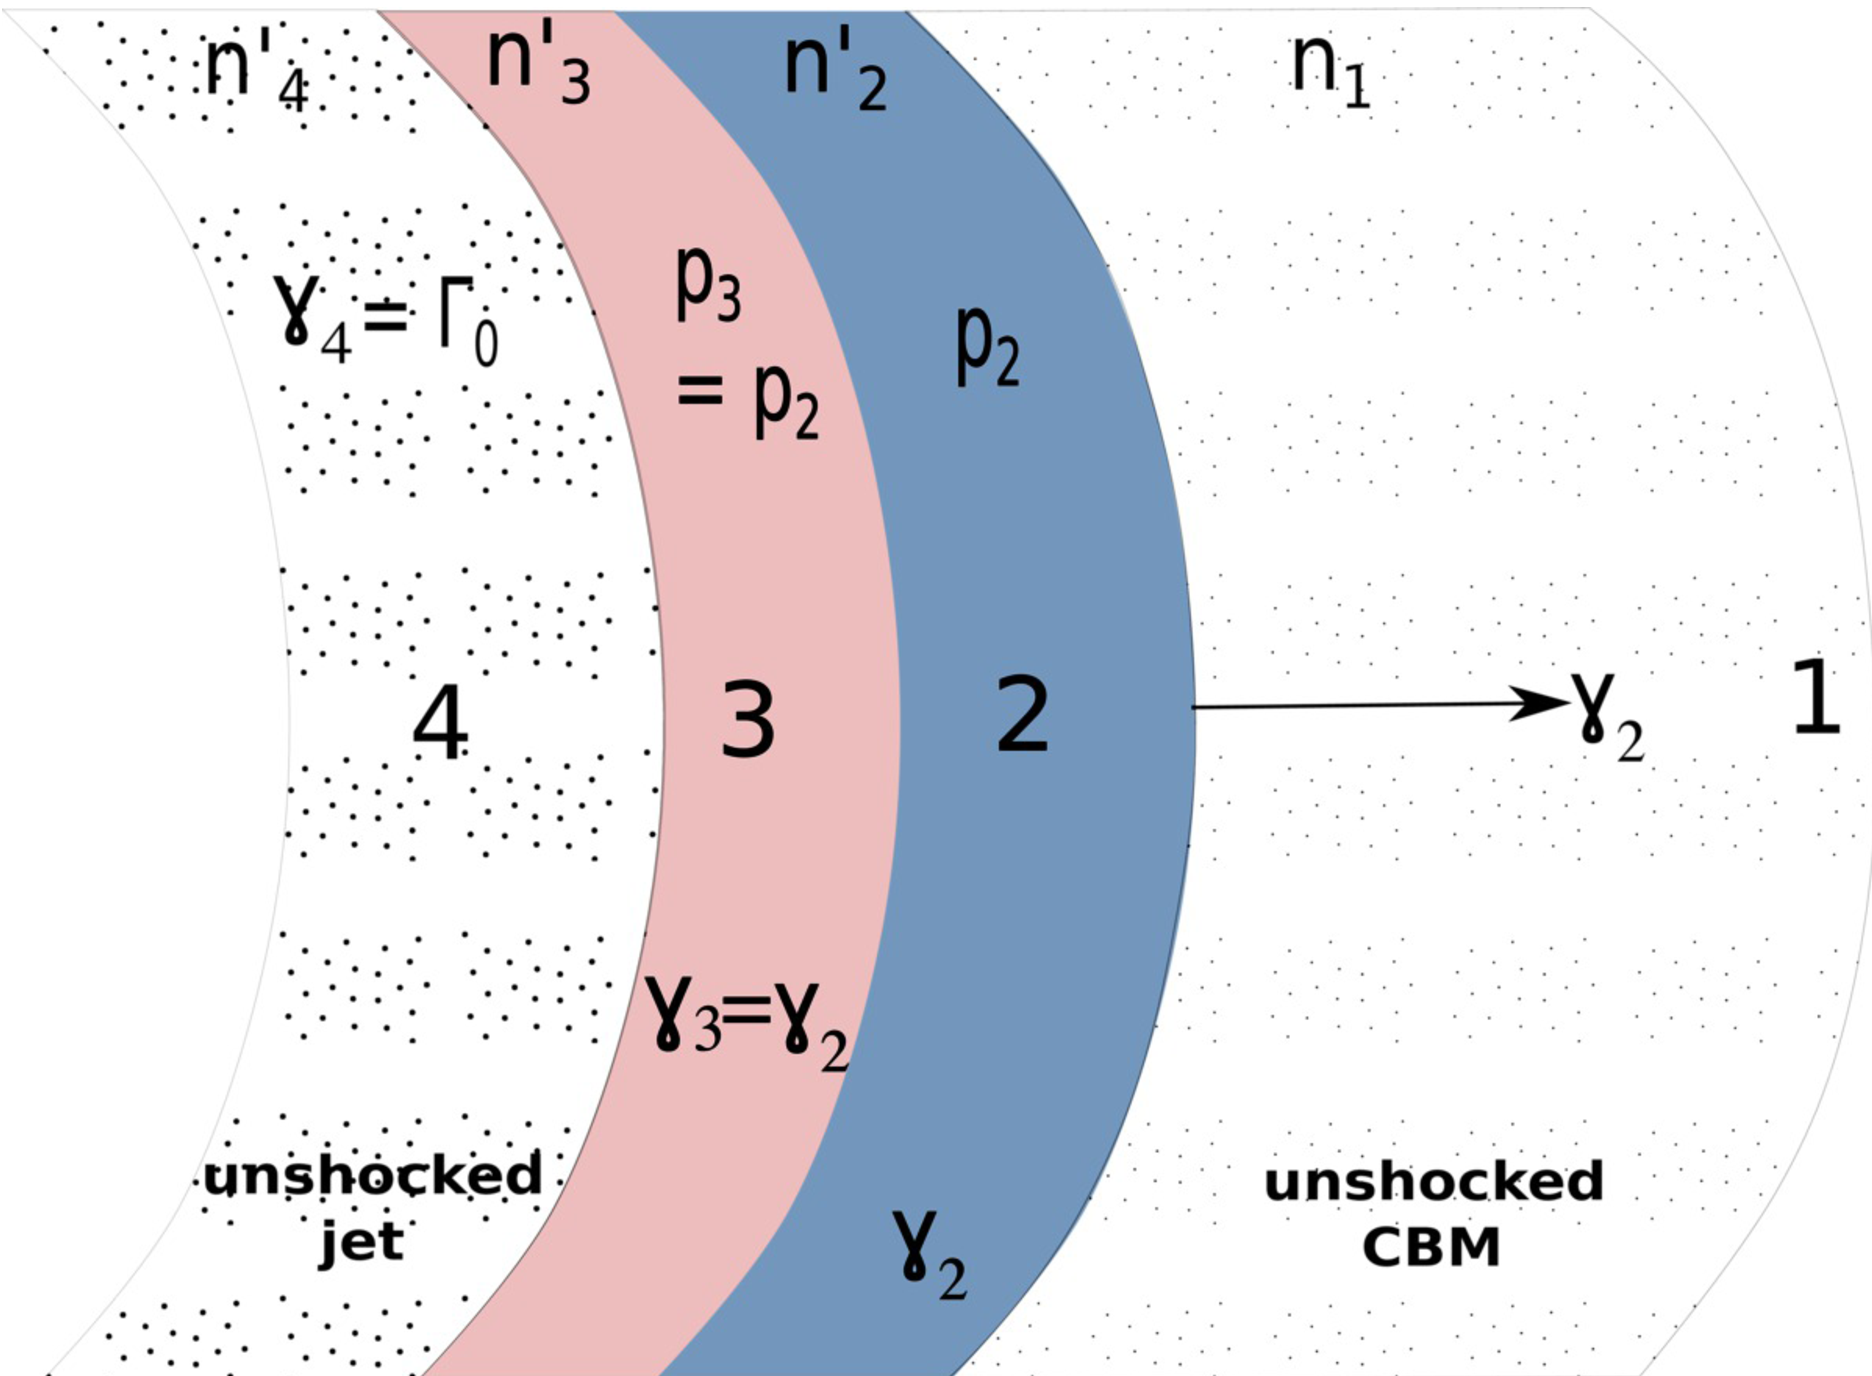
\includegraphics[width=0.45\textwidth]{Fig_8_KZ.pdf}
%    \caption{
%        This is a schematic sketch of a pair of shocks produced when a relativistic
%        jet from a \ac{GRB} collides with the \ac{CBM}, as viewed from the
%        rest frame of unshocked \ac{CBM}. Regions 2 \& 3 represent shocked \ac{CBM} and \ac{GRB}
%        jet respectively. They move together with the same \ac{LF} ($\gamma_2$, as viewed
%        by a stationary observer in the unshocked \ac{CBM}), and have the same pressure but
%        different densities.
%        (Adapted from \citet{Kumar:2014upa}, Fig.~8)
%    }
%    \label{fig:aafg:theory:sr8}
%\end{figure*}
%%
%Here, in Fig.~\ref{fig:aafg:theory:sr8} 
%\red{same as in Nava picture that you should put} the $2$ and $1$ subscripts 
%stand for downstream and upstream respectively, $e'$ is the internal energy density, 
%$n'$ is the proton number density, (both in the local fluid rest frame), 
%$\gamma_{21}$ is the relative \ac{LF} of plasma in region $2$ with respect to the 
%region $1$, $\gamma_{1s}$ is the relative \ac{LF} of plasma in region $1$ with 
%respect to the shock front and $\hat{\gamma}$ is the adiabatic index of the fluid.
%%
%For $\Gamma\gg1$ that usually describes early stage of the \ac{GRB} afterglow
%\citep{Piran:1999kx}, the $\hat{\gamma}=4/3$ 
%\red{recall that in subrelativistc it is $\hat{\gamma}=5/3$}
%%
%Then, $n_2'/n_1' = 3 ((4/3)\gamma_{21} + 1) = 4\gamma_{21} + 3 \approx 4\gamma_{21}$
%which implies that the downstream plasma is compressed with compression ratio
%$4\gamma_{21}$.
%%
%Similarly, approximating, the conservation equation 
%$\frac{e_2'}{n_2'} \approx \gamma_{21} m_p c^2$ and the last equation can be 
%simplified to $\gamma_{1s} \approx \sqrt{2} \gamma_{21}$, which implies that the 
%shock front travels faster then the downstream fluid.
%%
%Next, consider the self-similar deceleration phase of the blast wave in the 
%constant density \ac{CBM}. There, the energy conservation reads 
%%
%\begin{equation}
%E = \frac{4 \pi }{3 } R^3 n m_p c^2 \Gamma^2 = \text{ const}
%\end{equation}
%%
%where $\Gamma = \gamma_{21}$ is the \ac{LF} of the blastwave with respect to the 
%unshocked medium, $R$ is the radius of the blast wave (from \ac{CoE}). 
%%
%Note, that in the comoving frame the average proton thermal energy is 
%$m_p c^2 \Gamma$. In the lab frame it is $m_p c^2 \Gamma^2$. 
%Overall, we observe that $\Gamma^2 R^3 = \text{ const}$ or 
%%
%\begin{equation}
%\Gamma \propto R^{-3/2}
%\end{equation}
%%
%Now, consider the elapsed time in the observer frame. 
%As both the blast wave and emitted photons are moving in the same direction with the speed difference of $\sim 1/2 \Gamma^2$, 
%%
%\begin{equation}
%t_{obs} \sim \frac{R}{2\Gamma^2 c} \propto R^4 \propto \Gamma^{-8/3}
%\end{equation}
%%
%and 
%%
%\begin{equation}
%\Gamma \propto R^{-3/2} \propto t_{obs}^{-3/8}, \hspace{3mm} R\propto t_{obs}^{1/4}
%\end{equation}
%%
%
%%%______________________________________
%%% on the non-uniform CBM
%
%Next, we consider \red{power-law stratified density profile}, 
%
%\begin{equation}
%n = n_0 \Big(\frac{R}{R_0}\Big)^{-k}
%\end{equation}
%
%and obtain similar scaling relations.
%\red{I do not really need this. I can go directly to Peer model and Nava model}
%
%\begin{equation}
%E = \int n_0 \Big( \frac{R}{R_0} \Big)^{-k} m_p c^2 \Gamma^2  4\pi R^2 dR = \text{ const}
%\end{equation}
%
%where $R^{3-k} \Gamma^2 \text{ const}$. 
%
%After some derivation 
%
%\begin{equation}
%\Gamma\propto R^{(k-3)/2}\propto t_{obs}^{(k-3)/(8-2k)}
%\end{equation}
%
%And if $k=0$, the previously derived relation for constant density CBM follows.
%
%A particularly useful case is the \ac{CBM} filled with a free wind with constant mass loss rate $\dot{M}$ and wind speed $\upsilon_w$, that gives $\dot{M}=4\pi R^2 n \upsilon_w = \text{ const}$, or $n\propto R^{-k}$, \ie, the case of $k=2$ with $\Gamma\propto R^{-1/2}\propto t_{obs}^{-1/4}$.
%
%%%_______________________________________
%%% On the energy injection
%
%Now consider the case where the energy of the blast wave is continuously increasing. A possible physical scenario here is a long-lasting Poynting-flux dominated jet, feeding the fireball \gray{and suppressing the reverse shock}. 
%Then the energy of the outflow from the central engine has to be included into the energy equation of the blast wave
%
%\begin{equation}
%E_{tot} = E_0 + E_{inj}
%\end{equation}
%
%Consider a central engine with time dependent luminocity  $L(t) = L_0 (t_{obs}/t_0)^{-q}$. Then the energy equation reads
%
%\begin{equation}
%E_{tot} = E_0 + E_{inj} = E_0 + \int_{0}^{t_{obs}} L(t)dt = E_0 + \frac{L_0 t_0^q}{1-q}t_{obs}^{1-q}
%\end{equation}
%
%where $E_0$ is the initial energy of the blast wave and $E_{inj}$ is the injected energy into the blast wave from the central engine.
%
%Consider the case when energy injection increases with time noticeably, $q<1$.
%
%Then, when $E_{inj} \gg E_0$ for $q<1$, the blast wave scaling 
%
%\begin{equation}
%E_{tot} \sim E_{inj} \propto t_{obs}^{1-q}.
%\end{equation}
%
%and for the constant density \ac{CBM}, $\Gamma^2 R^3 \propto t_{obs}^{1-q}$ which eventually leads to $\Gamma\propto R^{-(2+q)/(4-2q)}\propto t_{obs}^{-(2+q)/8}$.
%
%And it is easy to see that if $q\rightarrow 1$, the 'no injection' case is resored.
%
%%%____________________________________
%%% Lorentz factor stratification of the ejecta as the Energy injection
%
%The energy can be added to the blast wave in a form of velocity stratified ejecta, when the wave decelerates, \eg,
%
%\begin{equation}
%E\propto \gamma^{1-s}\propto\Gamma^{1-s}
%\end{equation}
%
%where $\gamma$ is the \ac{LF} of the ejecta and $\Gamma$ is the \ac{LF} of the blast wave.
%Here the effects of the reverse shock can also be neglected as energy injection comes when $\Gamma\sim\gamma$ \red{[How does this work in the Peer/Nava model?]}
%
%This method is equivalent to the long-lived central engine with time dependent luminosity (at least for the dynamics of the blast wave), and the coefficient $s$ can be expressed in terms of $q$ \cite{Zhang:2005fa}. 
%
%For a uniform density \ac{CBM} the scaling relation reads
%
%\begin{equation}
%\Gamma\propto R^{-3/(1+s)}\propto t_{obs}^{-3/(7+s)}, \hspace{3mm} R\propto t_{obs}^{(1+s)/(7+s)}
%\end{equation}
%
%which then gives $s = (10-7q)/(2+q)$ and $q=(10-2s)/(7+s)$
%
%\red{The question is, can I add L(t) to the dE/dr of the Nava model and it is all?..}

%
%%%% ------------------
%%%% Shortened
%%%% ------------------
%
A universal part of the afterglow theory is the dynamics of the \trans{} 
\blast{} propagating through the \ac{ISM}, that is also called "fireball".
%
The theory of relativist shocks with applications to \ac{AGN} jets was 
developed by \citep{Blandford:1976}. Later, the theory was successfully 
applied to \ac{GRB} afterglows \citep{Costa:1997cg,vanParadijs:1997wr,Frail:1997qf},
and \ac{kN} afterglows \citep[\eg]{Nakar:2011cw,Hotokezaka:2015eja,Hotokezaka:2018gmo}.
%%
%Consider a \blast{} propagating though the cold \ac{CBM} with a power-law
%density profile, $n(R)$ with a \ac{LF} $\Gamma$.
%%
%The the total energy in the shocked plasma then is 
%$E \approx \frac{4\pi A R^{3-k}c^2 \Gamma^2}{3-k}$
%where $n(R) \propto AR^{-k}$ is the density of the \ac{CBM} at radius $R$ and 
%$4\pi A R^{3-k}/ (3-k)$ is the total swept up mass.
%%
%The conservation of the total energy governs the dynamics of the \blast{}. 
%The point at which the \ac{LF} and energy of the \blast{} decreases by half, and when 
%is referred to as \textit{deceleration radius}, $R_d$. \red{IS it?}.
%%
%Passing through the cold \ac{CBM}, shock front randomizes the velocity vectors,
%of particle, protons, raising their thermal energy, while their \ac{LF} remains
%unchanged. Additionally, shock compresses the plasma and accelerates the inbound 
%particles to a power-law distribution function, and amplifies the magnetic fields. 


Consider a relativistic shock propagating into a cold upstream medium.
The evolution of physical properties of the shock is governed by three conservation
laws: baryon number, $n' \Gamma c$, energy and momentum fluxes across the shock front.
The latter two are a embedded into the fluid energy momentum tensor 
Eq.~\eqref{eq:theory:tmunu_perf}.
%
%\begin{equation}
%T^{\mu\nu} = (\rho' c^2 + p') u^{\mu} u^{\nu} + p' g^{\mu\nu},
%\end{equation}
%
These equations can be written as 
%
\begin{equation} % subequations
    \begin{aligned} % align
    \frac{e_2'}{n_2'} &= (\gamma_{21} - 1)m_p c^2 \\
    \frac{n_2'}{n_1'} &= \frac{\hat{\gamma}\gamma_{21} + 1}{\hat{\gamma}-1} \\
    \gamma_{1s}^2 &= \frac{(\gamma_{21} + 1) [\hat{\gamma}(\gamma_{21}-1)+1]^2}{\hat{\gamma}(2-\hat{\gamma})(\gamma_{21}-1)+2}
    \end{aligned} % align
    \label{eq:afterglow:blast}
\end{equation} % subequations
%
\begin{figure*}[t]
    \centering 
    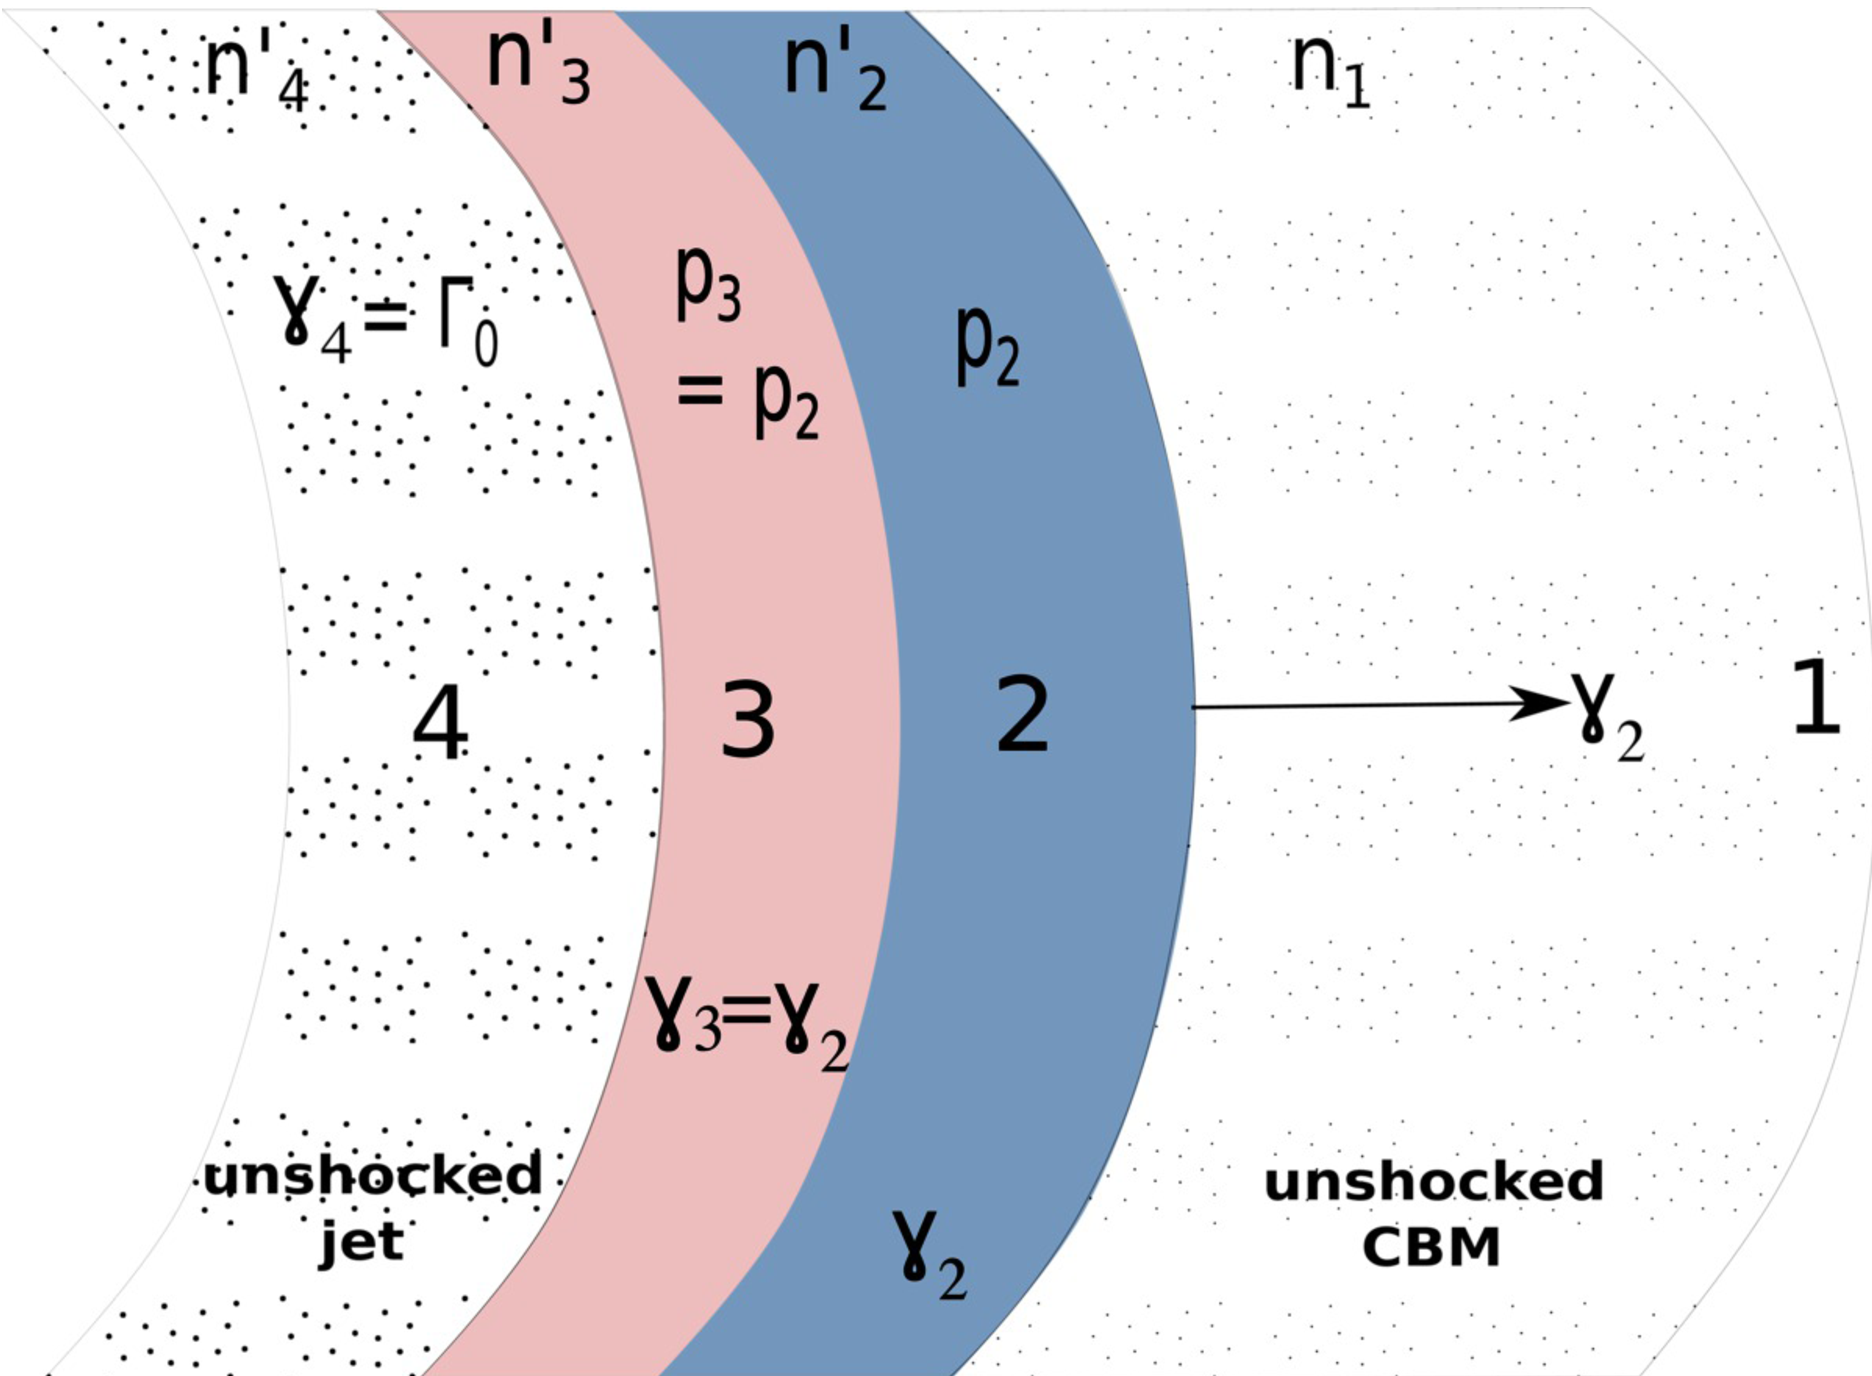
\includegraphics[width=0.45\textwidth]{Fig_8_KZ.pdf}
    \caption{
        This is a schematic sketch of a pair of shocks produced when a relativistic
        jet from a \ac{GRB} collides with the \ac{CBM}, as viewed from the
        rest frame of unshocked \ac{CBM}. Regions 2 \& 3 represent shocked \ac{CBM} and \ac{GRB}
        jet respectively. They move together with the same \ac{LF} ($\gamma_2$, as viewed
        by a stationary observer in the unshocked \ac{CBM}), and have the same pressure but
        different densities.
        (Adapted from \citet{Kumar:2014upa}, figure~8)
    }
    \label{fig:aafg:theory:sr8}
\end{figure*}
%
where subscripts $2$ and $1$ stand for downstream and upstream respectively, 
$e'$ is the internal energy density, $n'$ is the proton number density, 
$\gamma_{21}$ is the relative \ac{LF} of plasma in region 
$2$ with respect to the region $1$
$\gamma_{1s}$ is the relative \ac{LF} of plasma in region $1$ with respect to the shock front,
$\hat{\gamma}$ is the adiabatic index of the fluid, for the ideal, relativistic 
fluid is $\hat{\gamma}=4/3$ and subrelativisitc $\hat{\gamma}=5/3$.
The $2$ and $1$ regions are also shown in Fig.~\ref{fig:aafg:theory:sr8} 
(see also \cite{Nava:2013} for a more comprehensive take).
%
Solving the system Eq.~\eqref{eq:afterglow:blast} gives the full evolution 
of the \blast{}. 


%\subsection{Afterglow synchrotron emission}

\section{Method}

\def\eq{\text{equation}}
\def\eqs{\text{equations}}

We calculate the non-thermal 
radiation arising from the dynamical ejecta propagating into the cold \ac{ISM} 
with the semi-analytic code \texttt{PyBlastAfterglow}. 
%
Initial data for the dynamical evolution is taken from the \ac{NR} ejecta 
profiles for the mass as a function of energy and velocity, that is 
are used to compute the kinetic energy distributions 
(See Ch.~\ref{ch:bns_sims} and Fig.~\ref{fig:ejecta_vel_hist}).
%
Then, the adiabatic radial expansion of the ejecta in the thin shell approximation 
at each polar angle using the kinetic energy distributions.
%
We adopt the \blast{} dynamics formalism from \citet{Nava:2013} that cast the 
Eqs.~\eqref{eq:afterglow:blast} as a set of \acp{ODE} for the \blast{} \ac{LF},
swept-up mass and energy. The system is then solved via 
4th order adaptive step \ac{RK} method.
The effects of radiation losses, discussed in \citet{Nava:2013} and lateral 
spreading of the \blast{}, \citep[\eg][]{Granot:2012} are turned off.
%
The adiabatic index, $\hat{\gamma}$, is computed from the approximation to the 
numerical study of the \trans{} fluid \citep[\eq~5 in][]{Service:1986} as a function 
of normalized temperature \citep[\eq~11 in][]{Peer:2012}. It smoothly connects the 
$\hat{\gamma}=4/3$ and $\hat{\gamma}=5/3$ regimes. 

We adopt a dommon assumption that a fixed fraction of the \blast{} energy is being
deposited into the electrons, $\varepsilon_e$, and magnetic field, $\varepsilon_B$, 
\citep[\eg][]{Dermer:1997pv}. 
The injected electrons distribution function is Eq.~\eqref{eq:afterglow:elec_dist},
with $p$, the spectral index, being a free parameter.
%
We compute the characteristic \acp{LF}, $\gamma_c$ and $\gamma_m$ using the standard
prescriptions \citep[\eqs~A3 and A4 in][respectively]{Johannesson:2006zs}.

The synchrotron emission in the comoving frame, Eq.~\eqref{eq:afterglow:sync_power},
is approximated with the smooth broken power-law  
\citep[\eqs~A2 and A6 in][respectively]{Johannesson:2006zs}, and the 
the characteristic frequencies are obtained from the characteristic \acp{LF} 
$\gamma_{m}$ and $\gamma_c$ via their \eq~A5.
%
%The synchrotron self-absorption is included via flux attenuation \citep[\eg][]{Dermer:2009}. %
%However, for the applications discussed in this paper, the self-absorption is not 
%relevant as the ejecta remains optically thin for the emission ${\geq3}\,$GHz 
%\citep[\eg][]{Piran:2012wd}.
%

The flux in the observer frame is obtained by itegrating over the \ac{EATS}, 
that are obtained by comping the $t_{obs}$ Eq.~\eqref{eq:afterglow:tobs} for each
segment. The relativist effects are taken into account via 
Doppler factor Eq.~\eqref{eq:afterglow:dop_fac}.
See \citet{Salmonson:2003} for the detailed discussion of the method, 
and \citet{Lamb:2018ohw,Fernandez:2021xce} for the recent implementations


\subsection{Method verification}

In order to verify the code performance and results we compare it to the results 
published in literature. Specifically, we consider code designed by \citet{Hotokezaka:2015eja},
and applied to the \ac{BNS} merger ejecta in \citet{Radice:2018pdn}.

\begin{figure}%%[t]
    \centering 
    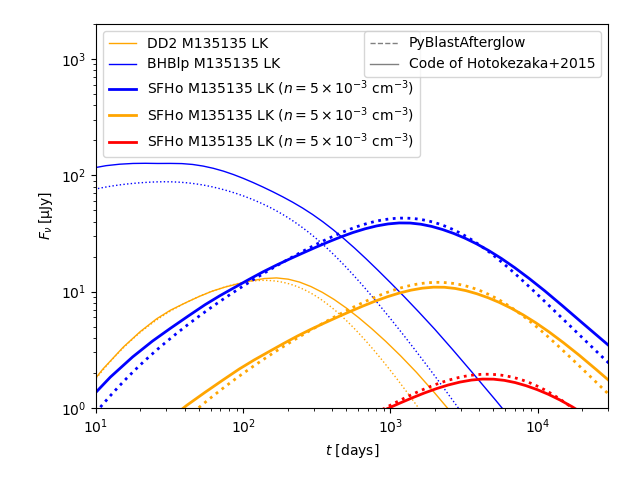
\includegraphics[width=0.49\textwidth]{ejecta_afterglow_vs_hotokezaka.png}
    \caption{
        Cumulative kinetic energy distribution for a selected set of models (\textit{top panel}) 
        and its angular distribution for a BLh $q=1.00$ model (\textit{bottom panel}).
        %% Also shown as a solid black line is the slow quasi-spherical model of \cite{Mooley:2017enz}.
        The vertical light green line marks the $\upsilon_{\text{ej}}=0.6$.
        The top panel shows that equal mass models have a more extend high energy tail,
        while the bottom panel shows that the angular distribution of the ejecta is not 
        uniform.
    } 
    \label{fig:afg_test}
\end{figure}

In Fig.~\ref{fig:afg_test} we show the \ac{kN} afterglow \acp{LC} from 
figures~30 and 31 of \citet{Radice:2018pdn}. The plot shows that that two codes
are in a good agreement. The discpeancies opserved can be attributed for different 
physical treatment of the \blast{} dynamics and synchrotron radiation. 
Notably, considering the large uncertainties on microphysical parameters and 
ejecta properties (discussed below) these discrepancies can be neglected.



\section{Results}

\begin{figure*}%%[t]
    \centering 
    %% ---\includegraphics[width=0.49\textwidth]{./figs/scatter_lightcurve_peaks.pdf}
    %% \includegraphics[width=0.48\textwidth]{./figs/xray_obs_representative_all_eos.pdf}
    %% \includegraphics[width=0.48\textwidth]{./figs/radio_obs_representative_all_eos.pdf}
    %% --- \includegraphics[width=0.49\textwidth]{./figs/scatter_q_lam_ideaplot.pdf}
    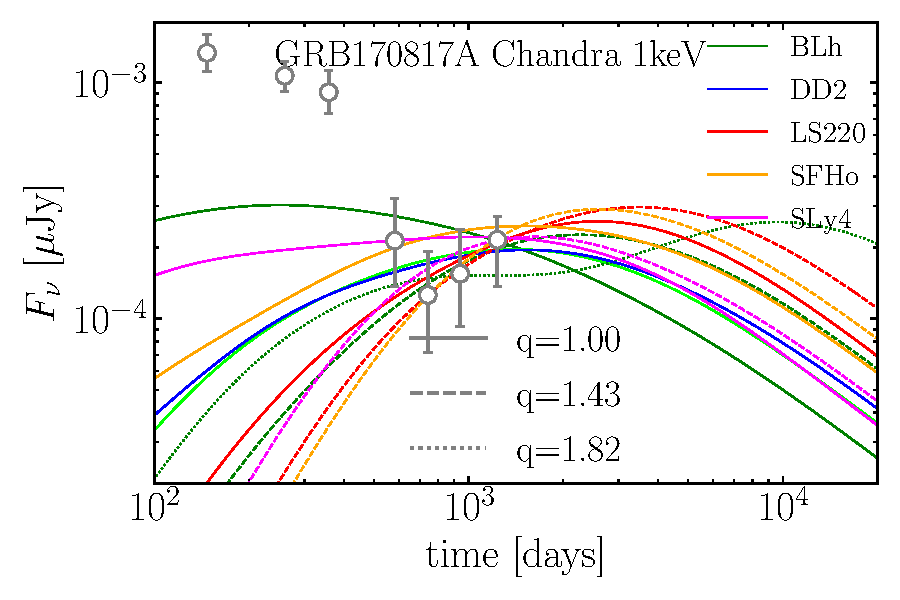
\includegraphics[width=0.48\textwidth]{kn_afterglow/best_xray_obs_representative_all_eos.pdf}
    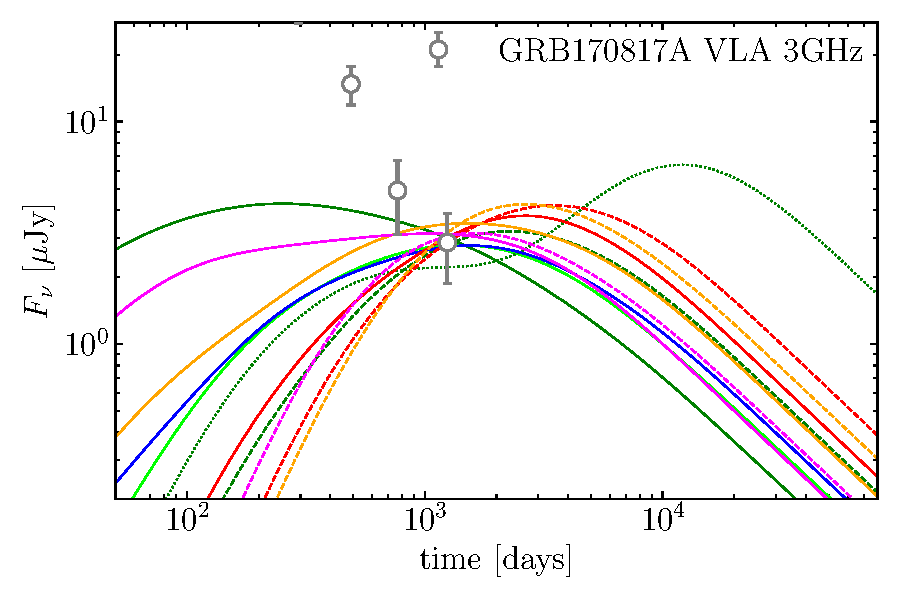
\includegraphics[width=0.48\textwidth]{kn_afterglow/best_radio_obs_representative_all_eos.pdf}
    \caption{
        Representative kilonova afterglow \acp{LC} for \ac{NR} models, 
        in X-ray (\textit{left panel}) and in radio (\textit{right panel}), where 
        %% There, every marker is annotated with two numbers, the tops is the peak time in years and the bottom is the peak flux in nJy ($10^{-9}$~Jy). The red color means that the value is below latest observations, that are $t=3.31$~years and $F_{\nu}=0.34$~$n$Jy. And the green color means that the model peak values are above the observational lower limit. 
        the gray circles are the observational data from \citet{Hajela:2021faz,Balasubramanian:2021kny}.
        %% The gray circles are the observational  in the X-ray band $0.3-10$~keV obtained from \citet{Fong:2017ekk,Hajela:2019mjy,Hajela:2020}.
        The synthetic \acp{LC} are computed with varying 
        micrphysical parameters and \ac{ISM} density within the 
        range of credibility to achieve a better fit to observational data (see Tab.~\ref{tab:pars} for details).
        %% The synthetic \acp{LC} are computed with the following parameters: 
        %% $\epsilon_e = 0.1$, $\epsilon_B\in(10^{-3},10^{-2})$, $n_{\text{ISM}}\in(10^{-3},10^{-2})$~$\ccm{}$.
        %% The last two parameters are varied for each model to achieve a better fit to the data. 
        %% ---
        The plots show that, within allowed parameter ranges, the \acp{LC} 
        from all models are in agreement with observations. 
        Models with moderately stiff \ac{EOS} and $q<1<1.8$ are tentatively preferred,
        as their flux is rising at $t\geq10^3$~days, in agreement with observations.
        %% --- 
        %% The plot shows that while for all models the peak time and magnitude are
        %% relatively close to the X-ray observed data, the models with moderately stiff \ac{EOS} and $q<1<1.8$ are tentatively preferred. 
    } 
    \label{fig:lightcurves}
\end{figure*}

\begin{table}
    \begin{center}
        \caption{
            List of parameters for synthetic \acp{LC} shown in the Fig~\ref{fig:lightcurves} 
            and Fig.~\ref{fig:lightcurve_peaks}.
            For the former the microphysical and \ac{ISM} density are adjusted model-wise 
            to achieved the good agreement with observations. For the latter,
            (the last row of the table) the parameters are the same for all models shown.
            Other parameters, such as observational angle, are the same everywhere (see text).
            (Adapted from \citet{Nedora:2021eoj})
        }
        \begin{tabular}{l | l l l l}
            Fig~\ref{fig:lightcurves} & $p$ & $\epsilon_e$ & $\epsilon_b$ & $n_{\text{ISM}}$ \\ \hline 
            BLh q=1.00    & 2.05 & 0.1          & 0.002        & 0.005            \\
            BLh q=1.43    & 2.05 & 0.1          & 0.003        & 0.005            \\
            BLh q=1.82    & 2.05 & 0.1          & 0.01         & 0.01             \\
            DD2 q=1.00    & 2.05 & 0.1          & 0.005        & 0.005            \\
            LS220 q=1.00  & 2.05 & 0.1          & 0.01         & 0.005            \\
            LS220 q=1.43  & 2.05 & 0.1          & 0.001        & 0.005            \\
            SFHo q=1.00   & 2.05 & 0.1          & 0.001        & 0.004            \\
            SFHo q=1.43   & 2.05 & 0.1          & 0.01         & 0.005            \\
            SLy4 q=1.00   & 2.05 & 0.1          & 0.001        & 0.004            \\
            SLy4 q=1.43   & 2.05 & 0.1          & 0.004        & 0.005            \\ \hline
            Fig.~\ref{fig:lightcurve_peaks}  & 2.15 & 0.2         & 0.005        & 0.005           
        \end{tabular}
    \end{center}
    \label{tab:pars}
\end{table}

In order to compute the \ac{kN} afterglow \acp{LC}, several free parameters of the model
need to be set. Specifically, we consider the \ac{ISM} density to be uniform with 
$\nism\in(10^{-3}, 10^{-2})\,\ccm$ \citep{Hajela:2019mjy}. 
The observational angle, (the angle between the line of sight and the polar axis of the 
\ac{BNS} system is set to $\theta_{\text{obs}}=30$~deg \citep{TheLIGOScientific:2017qsa}.
The luminosity distance of NGC 4993, the host galaxy of \GW{} is  $41.3\times10^{6}$~pc 
with the redshift $z=0.0099$ \citep{Hjorth:2017yza}.
%
The index of the electron energy distribution, $p$, and microphysical parameters are 
chosed based on the recent observations of the \GRB{}, where the spectral evolution 
was detected \cite{Hajela:2021faz}.  (see however \citet{Troja:2021xsw}). 
%
We consider the 
$\varepsilon_e\in(0.1, 0.2)$,
$\varepsilon_B\in(10^{-3}, 10^{-2})$, 
$p\in[2.05,2.15]$.


In Fig.~\ref{fig:lightcurves} we show the \acp{LC} in X-ray and radio bands for several 
representative \ac{BNS} merger models together with latest \GRB{} observational data. 
%% --- lightcurve shape
Ejecta velocity and angular distribution defines primarily the shape of the \acp{LC}.
Specifically, \ac{BNS} models with ejecta that show broad velocity distribution 
(for example, models with SLy4 \ac{EOS} and $q=1$, shown in Fig.~\ref{fig:ejecta_vel_hist})
leads to a wide \ac{LC}, with an early rise time, comaptible with that of the early \GRB{}
afterglow. This behaviour is guverned by the deceleration of the fastest ejecta shells, 
emission from which peak early. If the velocity distribution is rather narrow, with most 
material moving at ${\leq}0.2$~c (such is the model with LS220 \ac{EOS} and $q=1.43$) 
the \ac{LC} rise is steeper and occurs later (${\sim}10^2$~days after merger). 

%% --- general agreement with observations
Notably, the \ac{kN} afterglow \acp{LC} of most models are in good agreement with the 
rebrightening of the \GRB{} within the uncertain microphsical parameters and \ac{ISM} 
density.
Specifically, this agreement is particularly good for models with moderately stiff 
\acp{EOS} and $1.00<q<1.82$, with respect to the \ac{LC} peak time.

\begin{figure}
    \begin{center}
    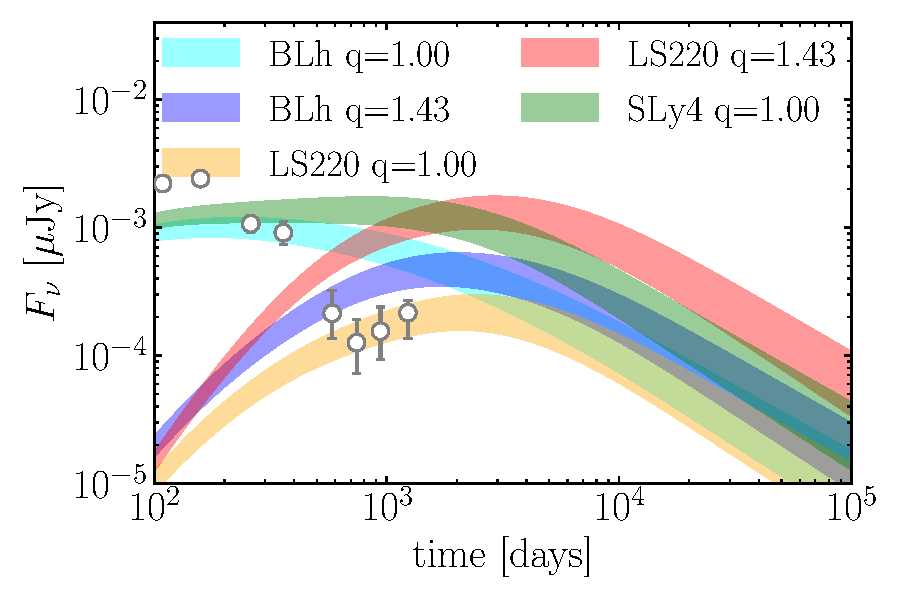
\includegraphics[scale=0.49]{kn_afterglow/KN-afterglow-NR-massratios.pdf}
    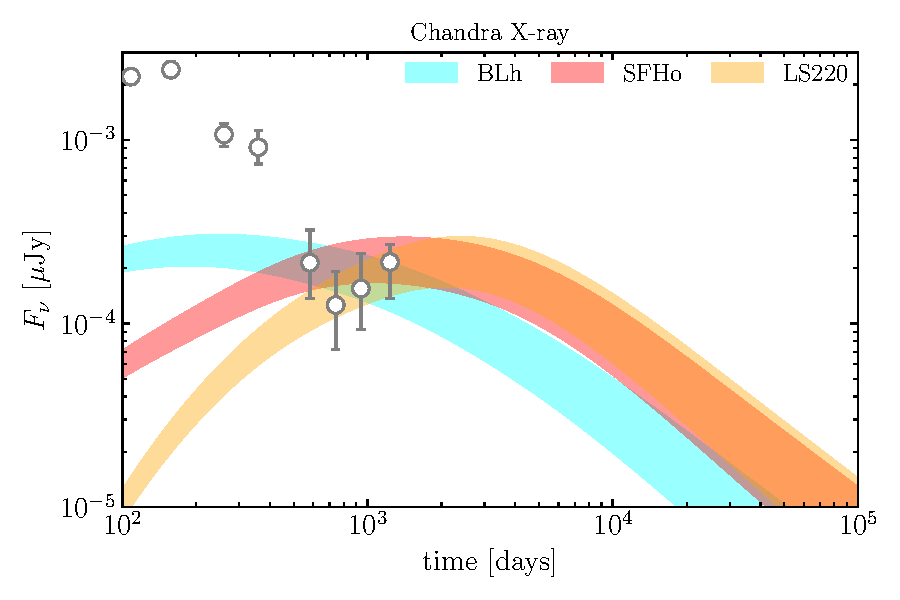
\includegraphics[scale=0.49]{kn_afterglow/KN-afterglow-NR-equalmass.pdf}
    \caption{
        The effect of the cahnging $p$ from $2.15$ (lower boundary of colored bands) to 
        $2.05$ (upper boundary of colored bands) shown in a set of \ac{kN} afterglow 
        X-ray \acp{LC} for \ac{DE} from a sample of \ac{NR} \ac{BNS} merger simulations.
        %% ---
        In \emph{upper panel} the models with different \mr{} are shown and the 
        $\nism=6\times10^{-3}$~cm$^{-3}$, and microphysical parameters, 
        $\varepsilon_{\rm e}=10^{-1}$, $\varepsilon_{\rm B}=10^{-2}$.
        %% --- 
        In \emph{lower panel} the models with $q=1$ are shown and afterglow
        parameters are adjusted to fit observations, 
        with $\varepsilon_{\rm e}=0.1$ fixed and  
        $\nism\sim 6\times 10^{-3}, 5\times 10^{-3},5\times 10^{-3}\,\rm{cm^{-3}}$
        $\varepsilon_{\rm B}\sim 10^{-2},2\times 10^{-3},10^{-3}$ for models with 
        LS220, BLh and SFHo \acp{EOS} respectively.
        (Adapted from \citet{Hajela:2021faz})\red{rephrased}
    }
    \end{center}
    \label{fig:kn_afterglow}
\end{figure}

From the \GRB{} model fitting the electron power law index $p$ is well constrain to $p=2.15$
\citep[\eg][]{Hajela:2019mjy}. The new emergent comonent in \ac{GRB} was found to have a lower 
$p=2.05$ \citep{Hajela:2021faz}. The effect of the decrease in $p$ is shown in 
Fig.~\ref{fig:kn_afterglow}. Notably, the parameters $p$, $\varepsilon_e$. $\varepsilon_b$ and 
$\nism$ are very degenerate, meaining that the change of one can be offset by the change in 
another withing these parameters' ranges of credibility. 

\begin{figure}%%[t]
    \centering 
    %%     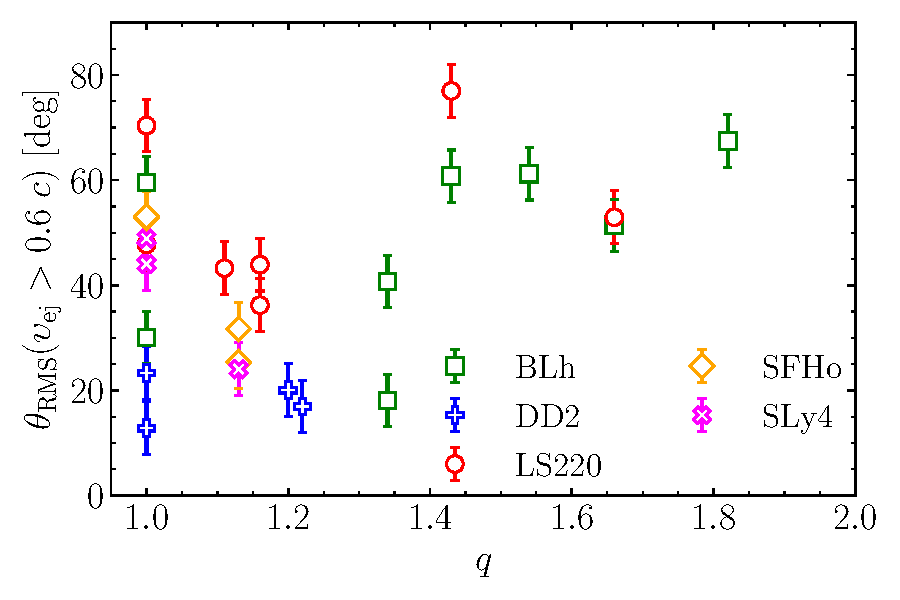
\includegraphics[width=0.49\textwidth]{./figs/scatter_thetarms_vej06.pdf}
    %% \includegraphics[width=0.49\textwidth]{figs/scatter_lightcurve_peaks_vs_lambda.pdf}
    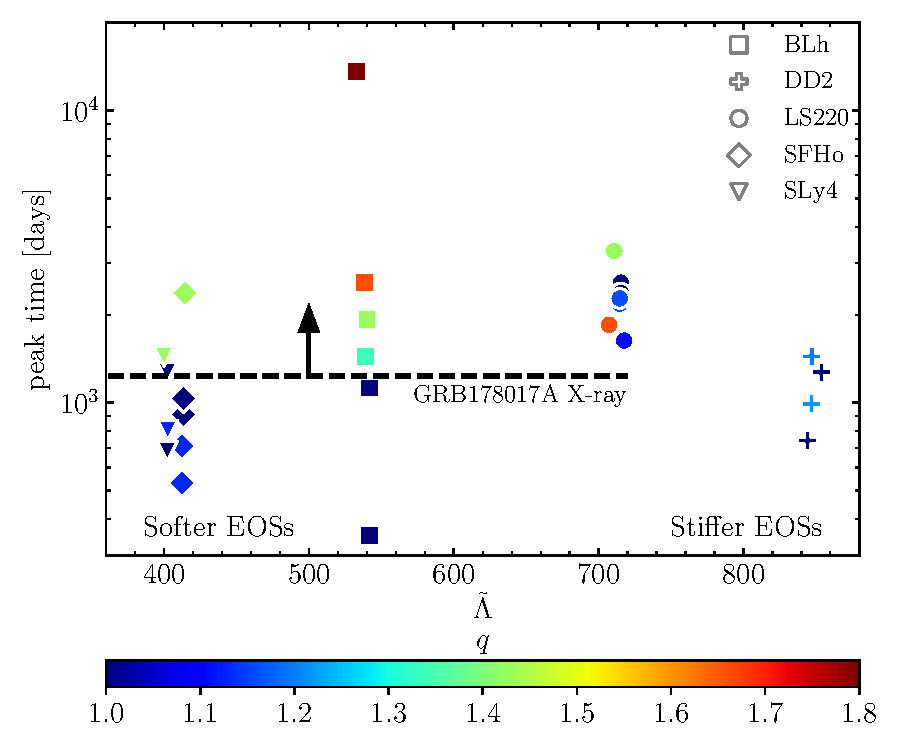
\includegraphics[width=0.49\textwidth]{kn_afterglow/scatter_lightcurve_tpeak_vs_lambda.pdf}
    \caption{
        Peak time, $t_p$, for \ac{LC} for all considered \ac{NR} simulations. 
        Dashed black line corresponds to the last observation of \GRB{} afterglow,
        where the rising flux implies that it is a lower limit on the kilonova 
        afterglow.
        The microphysical parameters and \ac{ISM} density for all models are fixed and 
        given in the Tab.~\ref{tab:pars}.
        The plot shows that in general the $t_p$ increases with mass ration and with 
        softness of the \ac{EOS}, except for the softest, DD2 \ac{EOS}. 
    } 
    \label{fig:lightcurve_peaks}
\end{figure}

%% --- Peak FLUX --- [UPDATED] --- IN CASE IT IS NEEDED [ BUT WITH NO FIGURE ]
If we fix the \ac{ISM} density and microphysical parameters to 
$\nism=5\times10^{-3}$~\gcm, $\varepsilon_e=0.1$ and $\varepsilon_b=5\times10^{-3}$, 
we observe that the \ac{LC} peak flux, $F_{\nu;p}$, is the highest for 
for soft \acp{EOS} such as SLy4. 
In general, however, we do not find a strong dependency between the \ac{EOS} and $F_{\nu;p}$.
With respect to the \mr{} we find that for models with sift \ac{EOS} the larger the \mr{},
the smaller the $F_{\nu;p}$. 
This behaviour can be attributed to the overall dependency of the ejecta mass-averaged 
velocity on the \mr{} (see Fig.~\ref{fig:ejecta:dyn:dsfits}).
As the mass-averaged velocity decreases when \mr{} increases, the 
total kinetic energy budget of these models rises \red{eh?}.
Slower, more massive ejecta have lower peak flux.
Notably, for the models with stiffer \acp{EOS} the dependency on \mr{} is not clear. 

%% --- UNCERTANTIES --- dominant --- microphysics 
%% It is however important to note that the \ac{LC} fluxes and the $F_{\nu,p}$ 
%% depend strongly on the shock michrophsyics. Within the error bars provided by 
%% \citet{Hajela:2019mjy}, they can vary by more then one order of magnitude.  
%% Additionally, the slope of the electron distribution, 
%% $p$, was shown to be lower for the emerging new component of \GRB{} afterglow 
%% (Hajela et al.~in prep). The change from $p=2.15$ to $p=2.05$ translates to the
%% inclrease in $F_{\nu,p}$ by $\sim2$.
%% --- uncertanties -- subdominat -- ejecta
We find that the the \ac{LC} shape and peak time do not depend strongly on the 
uncertain microphysical parameters and \ac{ISM} density. With respect to the latter, 
the peak time changes by a facter of a few when $\nism\in(10^{-3},10^{-2})~\ccm$.
Finite resolution effects that are present in ejecta properties do affect the 
afterglow \acp{LC}. Specifically, the $t_p$ changes by a factor of ${\leq2}$, 
and $F_{\nu;p}$ changes withing a factor of ${\leq4}$. However, our analysis 
shows that the uncertainty in $\nism,\,\varepsilon_e,\,\varepsilon_b$ and $p$ are larger. 
%% --- Robust feature
%% Specifically, the \ac{LC} shape and the peak time appear to be robust 
%% both with resolution and with microphysics, as they set by the dynamics 

%\section{Discussion}
%
%In this section we considered the synchrotron afterglow arising from the interaction 
%of \ac{DE} and \ac{ISM} for a set of \ac{NR} \ac{BNS} models. 
%%
%The recent observations of \GRB{} by Chandra, ${\sim}10^3$~days after the \GW{} event 
%showed the emergence of the rising flux component. Our analysis suggests that this 
%rebrightening can be attributed to the emergence of the \ac{kN} afterglow, as its 
%properties, such as time and flux are naturally reproduced by the \ac{kN} afterglow 
%from ab-initio \ac{NR} \ac{BNS} simulations.
%%
%In the analysis we evolved the \ac{DE} with semi-analytic code and computed its 
%synchrotron emission. 
%We found that the synthetic \acp{LC} are in agreement with the emerging new component 
%in the \GRB{} afterglow within the range of credibility of the microphisycal parameters 
%and of the \ac{ISM} density, $n_{\text{ISM}}$. 
%% The \ac{LC} shape and the time of the peak depends primarily on the 
%% ejecta velocity distribution. If massive fast ejecta component is present, the \ac{LC} 
%% is broader and peaks before $10^3$~days postmerger, while afterglow from 
%% the ejecta with small/absent fast tail peaks on the timescale of $>10^3$~days 
%% (see Fig.\ref{fig:lightcurves}). 

%% --- Note on the observations
%% The latest \GRB{} observations by Chandra \newtxt{(and possibly VLA)} 
%% at $1234$~days show a rising flux (Hajela \textit{et al.} (in prep.)). 

Comparing the \GRB{} observations and synthetic \acp{LC} we observe, that the 
rebrightening at $1243$~days after merger has the following implications:
the \ac{kN} afterglow peak should be (i) later and (ii) brighter than what is
currently observed. 
%
The condition (ii) is weak as the \ac{LC} peak flux is not well constrained due to 
uncertain microphysical parameters.
%% With respect to our models, the (ii) condition suggests that models soft \ac{EOS} and large \mr{} are disfavoured, 
%% as their $F_{\nu,p}$ is lower then the observations.
%% However, an increase in $\epsilon_B$ by a factor of $2$ changes this result.
The condition (i), however, is more robust from that point of view and allows to 
asses afterglow from which models is more supported by observations.

%% --- PEAK TIME 
We show the peak time of afterglow \acp{LC} of all our models in 
Fig.~\ref{fig:lightcurve_peaks}. There, the microphysical parameters and $\nism$ are fixed 
and listed in Tab.~\ref{tab:pars}, last row). 
We consider all models here, including those that do not have fast ejecta tail 
(see Sec.~\ref{sec:bns_sims:fast_de}) as they their ejecta is still energetic enough 
to produce bright afterglow. 
%
The \ac{LC} peak times are ${\sim}10^3$~days for all models that do not undergo the 
tidal disruption. The latter, model with BLh \ac{EOS} and $q=1.82$ produces massive and 
slow ejecta that is cahracteried by a late afterglow \ac{LC} peak ${\sim}10^4$~days.
%
Overall, we observe that the $t_{p}<10^3$~days for models with $q\sim1$ and 
$t_p>10^3$~days for models with larger \mr{}. This relation appears more prominent for 
models with soft \ac{EOS}, as the ejecta in these models has a strong controbution from 
a shocked, fast component when \mr{} is small.
The kinetic energy of the ejecta fast tail increases with the contribution from the 
shocked component. And the afterglow of faster, less massive ejecta peaks earlier 
\citep[\eg][]{Hotokezaka:2015eja}.
Indeed, the time of the \ac{LC} peak depends primarily on the ejecta 
dynamics, the so-called deceleration time \citep[\eg][]{Piran:2012wd}.
%% --- 
%% In the Fig.~\ref{fig:lightcurve_peaks} we show the peak time, $t_{p}$, for each model, 
%% alongside the lower limit (the time of the latest observation).
%% --- 
In Fig.~\ref{fig:lightcurve_peaks} we also show the time of the latest observation 
of the rising flux in \GRB{} (horizontal line). This provides the lower limit on $t_p$
on accordance with (ii).
Synthetic \acp{LC} of models with moderate amount of fast ejecta, \eg, models with 
\acp{EOS} of mild stiffness and \mr{}, lie above the limit, while models with very 
energetic fast tails, found $q=1$ models with very stiff \acp{EOS}, peak earlier. 
%% ---

%%%% <<< moved to overall conclusion >>>
%The main conclusion of our work is that the observed rising flux in the afterglow of \GRB{} 
%at $10^3$~days can be explained by the \ac{kN} afterglow produced by ejecta in 
%ab-initio \ac{NR} \ac{BNS} simulations targeted to \GW{}. 
%%% ---
%Specifically, models with moderately stiff \acp{EOS} and moderately large \mr{}, 
%that produce a mild amount of fast ejecta, are favored.
%%% ---
%Out results are subjected to uncertainties, the dominant among which are introduced 
%by ill-constrained microphysical parameters. 
% Additionally, the systematic effects due to the finite resolution, neutrino treatment 
%and \acp{EOS} might be important. 
%%% ---
%A larger set of observations, that allows for a better assessment of shock microphysics, 
%and a larger sample of high resolution \ac{NR} simulations are required to investigate 
%these uncertainties further. We leave this to future works.